\documentclass[12pt,a4paper]{book}
\usepackage[utf8]{inputenc}                                             % Codificación
\usepackage[spanish,es-tabla]{babel}                                    % Lenguaje español, Tabla n: 
\usepackage[T1]{fontenc}                                                % Agregar fuentes con acentos
\usepackage{amsmath}                                                    % Paquetes necesarios  para matemáticas
\usepackage{amsfonts}
\usepackage{amssymb}
\usepackage{makeidx}                                                    % Paquete para indices
\usepackage{graphicx}                                                   % Para manejar imagenes
\graphicspath{{imagenes/}}                                              % Ruta de las imagenes, solo escribir nombre de la imagen
\usepackage[top=1in, left=0.9in, right=1.25in, bottom=1in]{geometry}	% Margenes
\usepackage{lipsum}
\author{Julisa Verdejo Palacios}
\title{Tesis}
\date{}
%-------------------------------------------------------------------------------
%                            Paquetes adicionales                              %
%-------------------------------------------------------------------------------
%-------------------------------------------------------------------------------
%                                Paquetes extras                               %
%-------------------------------------------------------------------------------
\setcounter{secnumdepth}{3}
\setcounter{tocdepth}{3} 
\usepackage{amsthm}
\theoremstyle{definition}
\newtheorem{axiom}{Axioma} %[chapter]
\renewcommand\theaxiom{\Roman{axiom}}

\theoremstyle{definition}
\newtheorem{property}{Propiedad} %[chapter]

\theoremstyle{definition}
\newtheorem{corollary}{Corolario} %[chapter]

\theoremstyle{definition}
\newtheorem{theorem}{Teorema} %[chapter]

\usepackage{lipsum}												% Texto de ejemplo \lipsum[1-30]
\decimalpoint													% Punto decimal en lugar de coma
\spanishsignitems												% Viñetas en lugar de cuadros
\raggedbottom													% Eliminar molestos warnings

\usepackage{comment}											% Comentarios largos
\usepackage{pdfpages}											% Incluir portada echa en Inkscape
\usepackage{setspace}											% Interlineado
\usepackage{makecell}											% Para tablas
\usepackage{xcolor}												% Colores en tablas
\usepackage{colortbl}
\usepackage{booktabs,multirow}
\usepackage{nicematrix}
\usepackage{array}												% Necesario para algunas tablas
\usepackage[inline]{enumitem}									% Personalizar itemize
\usepackage{multicol}											% Item 2 columns
\usepackage{cite}                                               % Para contraer las citas

\definecolor{Red}{RGB}{255,191,191}								% Colores definidos por el usuario
\definecolor{lightgreen}{rgb}{0.8,1,0.8}

\usepackage[nottoc]{tocbibind}									% Bibliografia en table of contents

\usepackage[figuresright]{rotating}								% Rotar figuras con caption
\usepackage{subcaption}											% Subfiguras
%-------------------------------------------------------------------------------
%                            Comandos matematicos                              %
%-------------------------------------------------------------------------------
\usepackage{steinmetz}											% Para representar fasores
\usepackage{bm}													% Bold math  \bm command
\newcommand{\binomb}[2]{\genfrac{[}{]}{0pt}{}{#1}{#2}}
%-------------------------------------------------------------------------------
%                        Paquetes para hipervinculos                           %
%-------------------------------------------------------------------------------
\usepackage[hidelinks]{hyperref}								% Añade los bookmarks y le quita la caja roja, \url{}
\urlstyle{same}
%-------------------------------------------------------------------------------
%                           Estilos de encabezados                             %
%-------------------------------------------------------------------------------
\usepackage{fancyhdr, blindtext}								% Libreria para encabezados

\renewcommand{\chaptermark}[1]{\markboth{#1}{}}					% Capitulos y secciones en minusculas
\renewcommand{\sectionmark}[1]{\markright{#1}}

% Define the chapter format
\usepackage{titlesec}
\titleformat{\chapter}[display]
  {\normalfont\huge\bfseries}
  {\chaptertitlename\ \thechapter}
  {0ex}
  {\titlerule\vspace{1.5ex}\filleft}
  [\vspace{1ex}\titlerule] % Espacio después del título del capítulo

\fancypagestyle{normalstyle}{%
  \fancyhf{}													% Reinicial estilos de header y footer
	\fancyhead[LE,RO]{\thepage}
	\fancyhead[LO]{\nouppercase{\rightmark}}
	\fancyhead[RE]{\nouppercase{\leftmark}}
	\renewcommand{\headrulewidth}{0.4pt}
	\renewcommand{\footrulewidth}{0pt}
	\setlength{\headheight}{14.62pt}
}

\fancypagestyle{Resumen}{%
  \fancyhf{}													% Reinicial estilos de header y footer
	\fancyhead[LE,RO]{\thepage}
	\fancyhead[LO]{\nouppercase{Resumen}}
	\fancyhead[RE]{\nouppercase{Resumen}}
	\renewcommand{\headrulewidth}{0.4pt}
	\renewcommand{\footrulewidth}{0pt}
	\setlength{\headheight}{14.62pt}
}
%-------------------------------------------------------------------------------
%                            Libreria de codigos                               %
%-------------------------------------------------------------------------------
% Paquetes necesarios
\usepackage{listings}
\usepackage{xcolor}

% Colores para tablas
\definecolor{Gray}{RGB}{230,230,230}
\definecolor{Red}{RGB}{255,191,191}

% Colores personalizados
\definecolor{verde}{rgb}{0,0.6,0}
\definecolor{gris}{RGB}{253, 253, 253}
\definecolor{grisfuerte}{RGB}{140, 140, 140}

% Deficion de lenguajes perzonalizados

% Estilos MATLAB
\lstdefinestyle{MATLAB}{
	language=MATLAB,
	basicstyle=\linespread{1}\tiny\fontfamily{pcr}\selectfont,
	backgroundcolor=\color{gris},
	frame=single,
	frameround=tttt,
	rulecolor=\color{black},
	commentstyle=\color{verde},
	keywordstyle=\color{blue}, %magenta
	stringstyle=\color{grisfuerte},                  
	captionpos=t,                    
	breaklines=true,                       
	breakatwhitespace=false,
	showspaces=false,                
	showstringspaces=false,
	showtabs=false,
	keepspaces=true,
	columns=flexible,
	tabsize=4,   
}

\lstdefinestyle{VHDL}{
	language=VHDL,
	basicstyle=\linespread{1}\tiny\fontfamily{pcr}\selectfont,
	backgroundcolor=\color{gris},
	frame=single,
	frameround=tttt,
	rulecolor=\color{black},
	commentstyle=\color{verde},
	keywordstyle=\color{blue}, %magenta
	stringstyle=\color{grisfuerte},                  
	captionpos=t,                    
	breaklines=true,                       
	breakatwhitespace=false,
	showspaces=false,                
	showstringspaces=false,
	showtabs=false,
	keepspaces=true,
	columns=flexible,
	tabsize=4,
	upquote=true,
}


\lstdefinestyle{VHDL_TEXT}{
	language=VHDL,
	basicstyle=\linespread{1}\footnotesize\fontfamily{pcr}\selectfont,
	backgroundcolor=\color{gris},
	frame=single,
	frameround=tttt,
	rulecolor=\color{black},
	commentstyle=\color{verde},
	keywordstyle=\color{blue}, %magenta
	stringstyle=\color{grisfuerte},                  
	captionpos=t,                    
	breaklines=true,                       
	breakatwhitespace=false,
	showspaces=false,                
	showstringspaces=false,
	showtabs=false,
	keepspaces=true,
	columns=flexible,
	tabsize=4,
	upquote=true,
}


\lstdefinestyle{C}{
	language=C,
	basicstyle=\linespread{1}\tiny\fontfamily{pcr}\selectfont,
	backgroundcolor=\color{gris},
	frame=single,
	frameround=tttt,
	rulecolor=\color{black},
	commentstyle=\color{verde},
	keywordstyle=\color{blue}, %magenta
	stringstyle=\color{grisfuerte},                  
	captionpos=t,                    
	breaklines=true,                       
	breakatwhitespace=false,
	showspaces=false,                
	showstringspaces=false,
	showtabs=false,
	keepspaces=true,
	columns=flexible,
	tabsize=4,
	upquote=true,    
}

\renewcommand{\lstlistingname}{Código}% Listing -> Algorithm
\renewcommand{\lstlistlistingname}{Índice de códigos}% 

%-------------------------------------------------------------------------------
%                           Caption en negritas                                %
%-------------------------------------------------------------------------------
\usepackage[labelfont=bf]{caption}
\captionsetup{labelfont=bf}


%-------------------------------------------------------------------------------
%                             Archivos a incluir                               %
%-------------------------------------------------------------------------------
\includeonly{
	portada,
	agradecimientos,
	resumen,
	ch1,
	ch2,
	ch3,
	ch4,
	ch5,
	ch6,
	Ap_A
}
%-------------------------------------------------------------------------------
%-------------------------------------------------------------------------------
\begin{document}
	
\includepdf[pages=-]{portada/main.pdf}

	\thispagestyle{empty}								            % Limpiar estilos de pagina

\frontmatter
\onehalfspacing										                % Desde este punto interlineado de 1.5
% 	\spacing{1.213}
	\chapter{Agradecimientos}

\begin{itemize}
\item A mi familia, mis padres Rafael y Pilar, mis hermanas Alejandra y Edith y a mi sobrino Diego, gracias por siempre estar al pendiente de mi, por motivarme a seguir adelante, por su amor y apoyo.
\item A mi compañero de vida y mejor amigo, Ciro Bermúdez, gracias por tu amor, comprensión y ternura.
\item A la Sra. Juana, gracias por su comprensión y por brindarme todo su apoyo en la recta final de mi trabajo.
\item A mis amigos, Juan, Yair, Javier, Hitan Divi, Nancy, Vicky y Jorge, gracias por sus consejos, apoyo y compañía.
\item A Intesc, gracias por brindarme soporte y asesoría.
\item A mis compañeros de laboratorio Victor y Julio, gracias por ayudarme resolviendo mis dudas y por hacer un ambiente agradable de trabajo.
\item A mi asesor, gracias por su paciencia y apoyo, el trabajo que realizamos juntos representa el inicio de mi carrera profesional.
\end{itemize}




\pagestyle{normalstyle}									            % Estilos de pagina personalizados
\tableofcontents            								        % Genera el índice
\addcontentsline{toc}{chapter}{\contentsname}

\listoffigures              								        % Indice de figuras
\listoftables               								        % Indice de tablas

\lstlistoflistings                                                  % Indice de códigos
\addcontentsline{toc}{chapter}{\lstlistlistingname}

	\chapter{Resumen}
    
    En esta tesis se diseñó e implementó un TRNG híbrido en la FPGA Xilinx Artix 7 xc7a35tcpg236-1 sobre la tarjeta de desarrollo Digilent Basys 3. Se utilizó un núcleo ERO-TRNG para generar una semilla de 64 bits que funciona como condición inicial para un mapa caótico bidimensional. Haciendo uso de la operación mod 256 se extraen 16 bits aleatorios por cada iteración del mapa. 

    En este trabajo se presenta toda la teoría necesaria para comprender los generadores de números aleatorios, así como su clasificación, fuentes de aleatoriedad, parámetros de evaluación pruebas estadísticas y arquitecturas de núcleos TRNG específicas para FPGA. Se estudian brevemente las características principales de los mapas caóticos como puntos fijos, estabilidad lineal, diagramas de bifurcación y diagramas de cobwebs. Después se expone la metodología de diseño para implementar en FPGA el mapa caótico bidimensional y el núcleo ERO-TRNG utilizando el lenguaje de descripción de hardware VHDL. El mapa caótico se implementó utilizando aritmética de punto fijo de 64 bits, 3 bits para la parte entera, 60 bits para la fraccionaria y un bit de signo y para comprobar su funcionamiento se empleó un simulador desarrollado lenguaje C. Posteriormente se analizó el dominio de atracción del mapa para diferentes parámetros con el fin de poder seleccionar un rango en que las condiciones iniciales produzcan caos, por ultimó se utilizaron multiplicadores de una sola constante para reducir el uso de recursos. Utilizando diversos elementos digitales básicos y el núcleo ERO-TRNG se diseñó un generador de semillas de 64 bits que alimenta a las condiciones iniciales del mapa caótico. Finalmente, las secuencias binarias obtenidas por el TRNG híbrido se mandaron a una computadora utilizando el protocolo de comunicación RS232 y se analizaron con las pruebas estadísticas NIST SP 800-22.

	\pagestyle{Resumen}	
	
\mainmatter
\pagestyle{normalstyle}	
	\chapter{Introducción}

Los sistemas de adquisición de datos (DAQs) son un conjunto de herramientas utilizadas para recopilar, procesar y analizar datos de fenómenos físicos. Los elementos básicos de un sistema de adquisición de datos incluyen sensores que capturan señales físicas, hardware de acondicionamiento de señales para procesar las salidas de los sensores, y una computadora que ejecuta software para adquirir y registrar los datos. 


El concepto de adquisición de datos se remonta a tiempos antiguos, cuando los seres humanos comenzaron a observar y registrar eventos naturales, como el movimiento de los cuerpos celestes, los cambios en el clima y el paso del tiempo. Las primeras civilizaciones desarrollaron métodos para la recolección de datos, como calendarios, instrumentos mecánicos, como el reloj solar, y libros de registros. Con la llegada de dispositivos analógicos y digitales, la adquisición de datos se hizo cada vez más sistemática y automatizada.


Algunos ejemplos de los sistemas de adquisición de datos aplicados en distintos sectores son: estaciones meteorológicas, utilizan DAQs para monitorear parámetros ambientales como la temperatura, la humedad, la velocidad del viento y la presión atmosférica. Estos sistemas suelen incluir sensores como termómetros, higrómetros y anemómetros, los datos se procesan y registran en ordenadores para hacer un seguimiento de los cambios climáticos. En la medicina, los electrocardiógrafos son un tipo de DAQs, miden la actividad eléctrica del corazón, procesan las señales y las muestran en forma de ondas en una pantalla. En la industria automotriz, durante la fase de desarrollo de los vehículos, los DAQs monitorean parámetros como el rendimiento del motor, la eficiencia del combustible y las emisiones de gases para garantizar el cumplimiento en los estándares de calidad y seguridad.


El uso de DAQs para la creación de imágenes con detectores infrarrojos, tiene múltiples aplicaciones, que van desde la seguridad y vigilancia en hogares \cite{Yii2023} hasta el ámbito médico, donde se utilizan para el diagnóstico de enfermedades como el cáncer de mama, diabetes \cite{LeneroBardallo2022} y patologías dermatológicas \cite{She2024}. También se emplean en la detección de gestos para dispositivos inteligentes \cite{LeBa2019} y en aplicaciones espaciales, como el monitoreo de las emisiones de dióxido de carbono en la atmósfera provocadas por la actividad humana \cite{Minoglou2019}. En la agricultura, para identificar las zonas del campo que sufren estrés hídrico o exceso de riego, lo que permite una mejor gestión del agua \cite{Parihar2021}.


Los detectores infrarrojos permiten capturar radiación que no es visible al ojo humano y la transforman en señales eléctricas que pueden ser medidas. Desarrollar un sistema de adquisición de datos para obtener imágenes infrarrojas es crucial, ya que estos sistemas interpretan las señales generadas por los detectores y las convierten en una imagen visible, proporcionando información valiosa sobre la distribución de la temperatura en un escenario específico.


Debido a la importancia de los sistemas de adquisición de datos en aplicaciones que utilizan detectores infrarrojos, es fundamental comprender el comportamiento de estos detectores. Conocer cómo responden a diferentes condiciones de luz y temperatura permite diseñar sistemas más eficientes y precisos para capturar imágenes térmicas.
    
    \section{Radiación Electromagnética}
    La radiación electromagnética es la emisión y transmisión de energía en forma de ondas electromagnéticas. El espectro electromagnético es una representación de los diversos tipos de radiación existentes, en él se definen los intervalos de longitudes de onda o frecuencia que cada una de ellas abarca \cite{Chang}.
            \begin{figure}[hbtp]
                \centering
                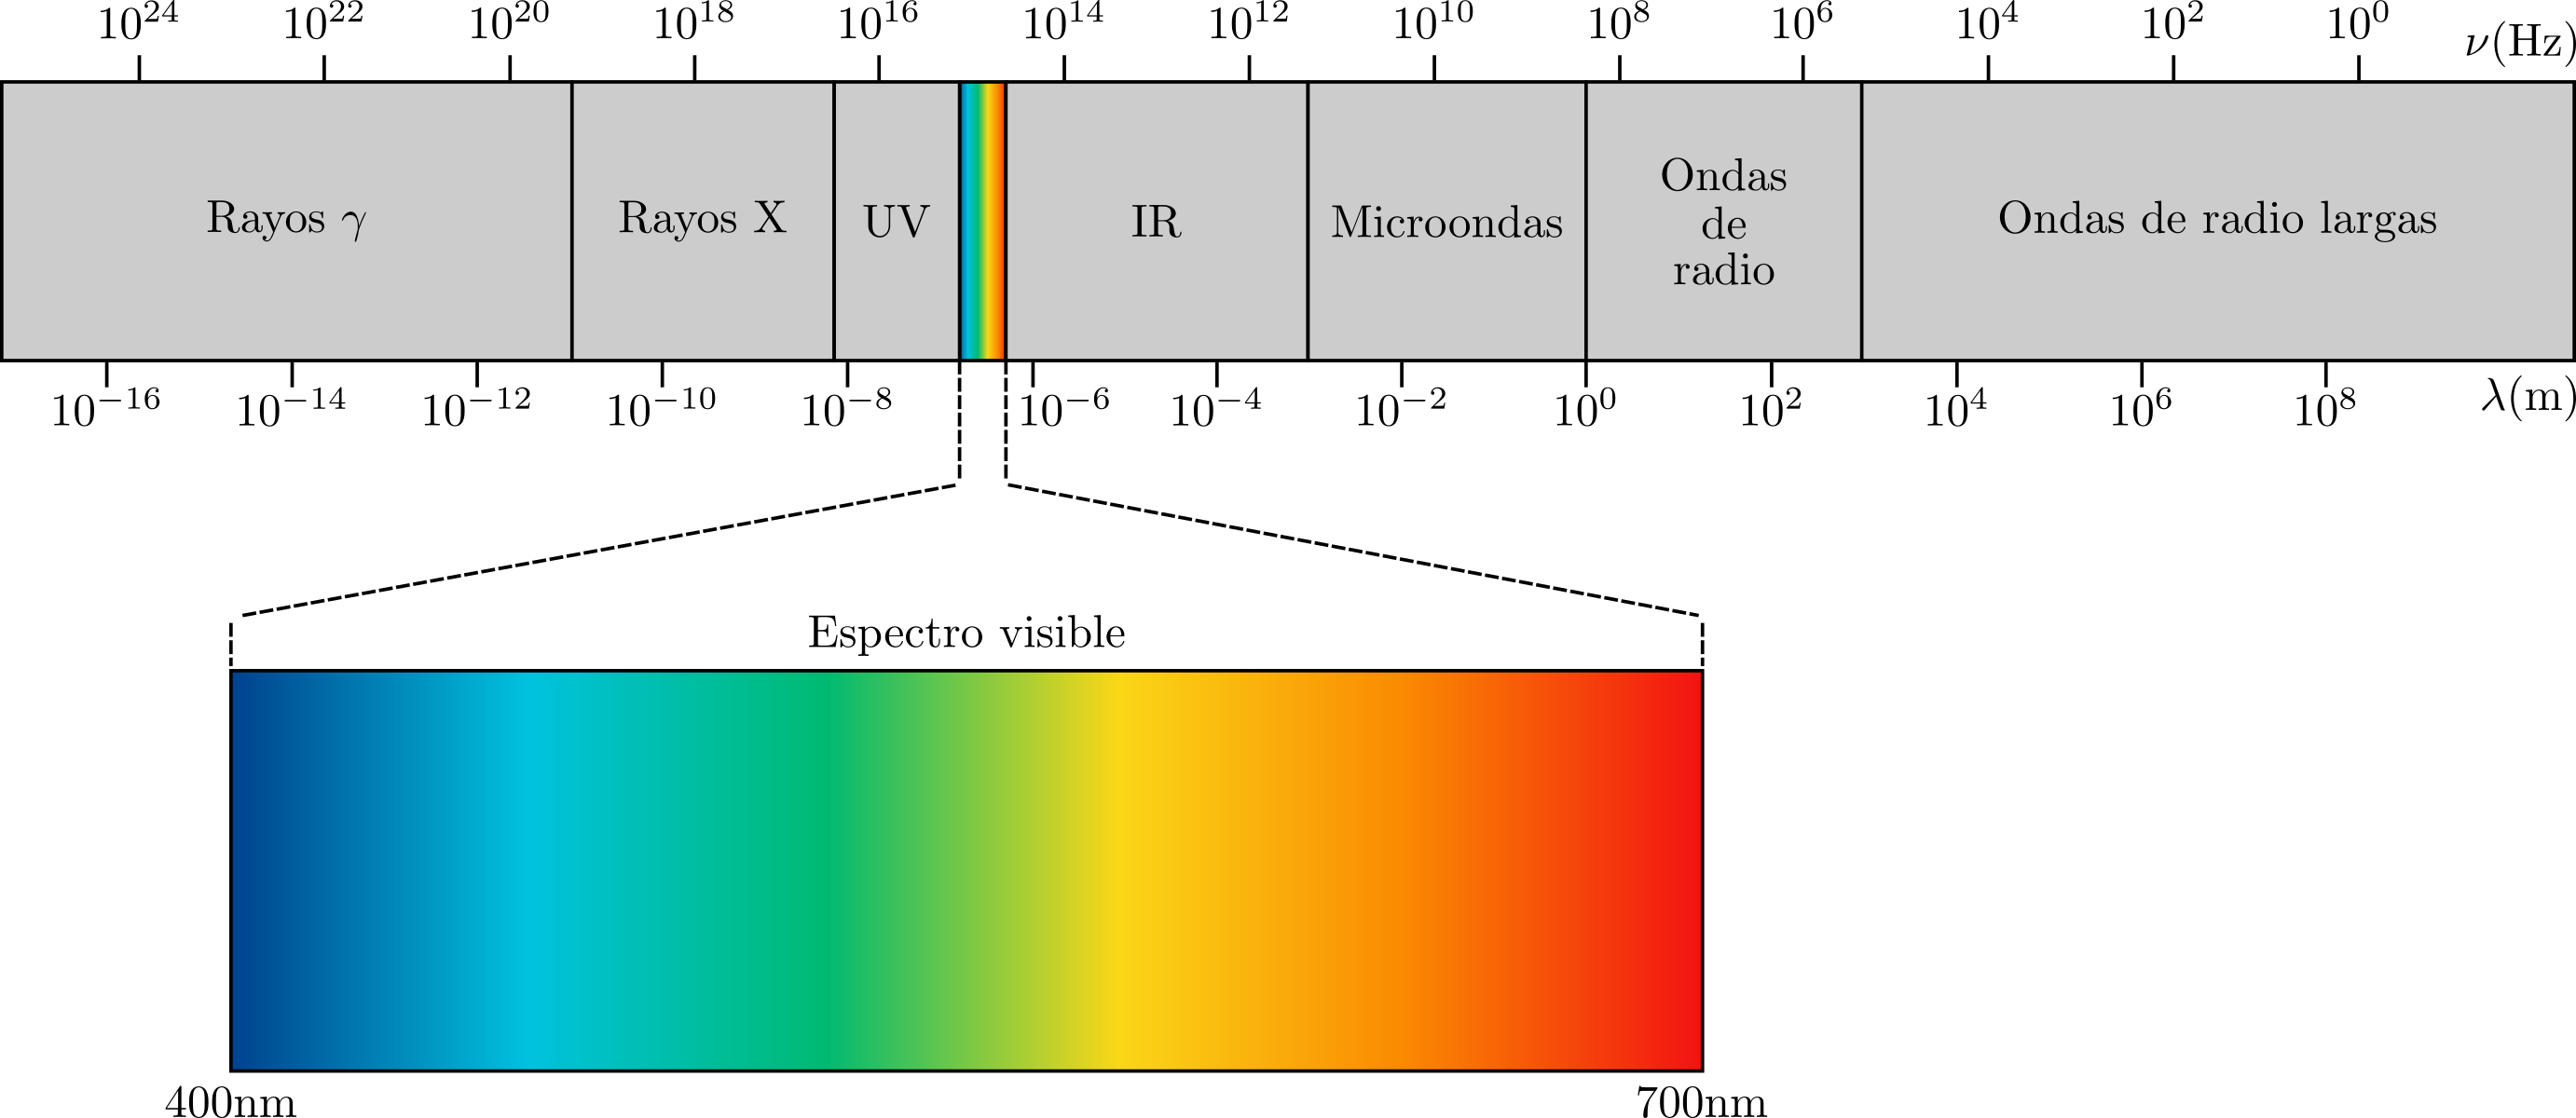
\includegraphics[width=0.8\textwidth]{espectro}
                \caption{Espectro electromagnético.}
                \label{fig:espectro}
            \end{figure}    
    
    Estas radiaciones obedecen las mismas leyes, la diferencia entre ellas radica en su longitud de onda o frecuencia, así como en la manera en que interactúan con los materiales ópticos, incluída la atmósfera \cite{Vincent}.
    
    Todos los cuerpos emiten radiación e.m  y debido al movimiento de sus átomos y moléculas se genera una temperatura en ellos. Los cuerpos con una temperatura mayor a 0K emiten radiación térmica por medio de ondas e.m. La radiación térmica es la radiación que emite un cuerpo por su temperatura \cite{Hollands}.
    
    La capacidad que tiene un cuerpo para emitir radiación está fuertemente relacionada con su capacidad de absorberla \cite{Beiser}.
    
    Una superficie ideal que absorbe toda la radiación que incide sobre él se denomina \textit{cuerpo negro} y el espectro de radiación que emite se llama \textit{radiación de cuerpo negro} \cite{Sears}.
    
    A pesar de que en la naturaleza no existe un objeto físico que pueda absorber toda la radiación incidente \cite{FUV3}, este puede representarse como un objeto hueco con una pequeña apertura donde cualquier radiación que incida en ella ingresa a la cavidad donde queda atrapada hasta que es absorbida \cite{Beiser}, \cite{FUV3}. En equilibrio térmico la radiación emitida por el cuerpo será exactamente igual a la absorbida.
    
    El cuerpo negro fue creado como una herramienta auxiliar para entender como los objetos emiten y absorben radiación.
    Hacia finales del siglo XIX la radiación de cuerpo negro ya había sido estudiada y dos leyes importantes sintetizaron los descubrimientos experimentales sobre este tema: La \textit{Ley de Stefan-Boltzmann} y la \textit{Ley de desplazamiento de Wien} \cite{FUV3}.
    
    La \textit{Ley de Stefan-Boltzmann} plantea que la intensidad de la radiación emitida por un cuerpo negro depende de su temperatura. La intensidad es proporcional a la cuarta potencia de la temperatura absoluta del cuerpo:
    
    \begin{equation}
        I = \sigma T^{4}
        \label{eq:Stefan-Boltzmann}
    \end{equation}
    donde:
    
    $T$ es la temperatura del cuerpo negro en K.
    
    $\sigma$ es la constante de Stefan-Boltzmann, $\sigma = 5.670\times10^{-8}\ W/m^{2}K^{4}$
    
    La intensidad de la radiación no se distribuye uniformemente a lo largo de todas las longitudes de onda. En cambio, su distribución puede medirse y describirse utilizando la intensidad por intervalo de longitud de onda, $I(\lambda)d\lambda$.
            \begin{figure}[hbtp]
                \centering
                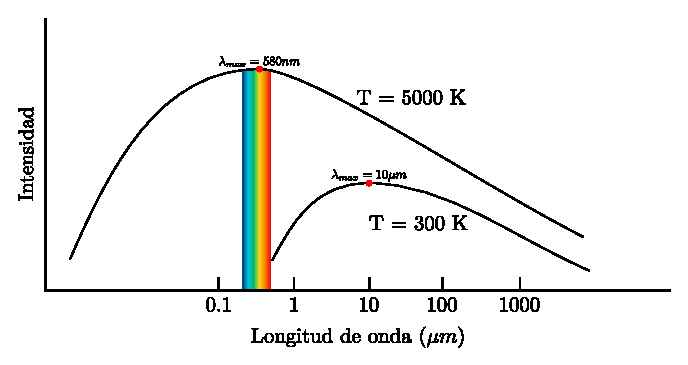
\includegraphics[width=0.8\textwidth]{intensidad_bb}
                \caption{Emitancia espectral de un cuerpo negro.}
                \label{fig:intensidad_bb}
            \end{figure}    
%    \newpage
    La Figura \ref{fig:intensidad_bb} muestra las intensidades registradas a dos temperaturas diferentes. En cada caso hay una longitud de onda específica $\lambda_{m}$ en la que la intensidad de la radiación emitida es máxima.
    
    La \textit{Ley de desplazamiento de Wien} indica que cuando la temperatura de un cuerpo negro aumenta, la longitud de onda en la que se emite la radiación máxima se desplaza hacia valores más cortos:
    
    \begin{equation}
        \lambda_{m} = \frac{2.90\times10^{-3}\ mK}{T}
        \label{eq:Wien}
    \end{equation}   
    donde:
    
    $\lambda_{m}$ es la longitud de onda en la que un cuerpo negro emite la mayor cantidad de radiación a una determinada temperatura \cite{Sears},\cite{FUV3}.
    
    De las leyes anteriores y la Figura \ref{fig:intensidad_bb} se puede deducir que la radiación UV, los rayos X y Gamma, son radiaciones más cálidas (radiaciones de alta energía), mientras que la radiación infrarroja está asociada a fenómenos con temperaturas cercanas a la temperatura ambiente \cite{Chang}, \cite{BlancoMDA}.     
    
    \section{Radiación Infrarroja} 
    La radiación infrarroja es un tipo de radiación electromagnética que cuenta con longitudes de onda mayores que las del rango visible. Se encuentra en el rango de 0.77$\mu m$ - 1$mm$ \cite{BlancoMDA}, y a su vez se divide en varias regiones las cuales se muestran en la Tabla \ref{tab:Div_IR} \cite{Rogalski}.
    
            \begin{table}[htbp]
                \caption{División de la radiación infrarroja.}
                \begin{center}
                    \resizebox{0.8\linewidth}{!}{ 
                    \begin{NiceTabular}{|l|c| }
                        \CodeBefore
                        \Body
                        \hline
                        \textbf{Region}  & \textbf{Rango de frecuencia ($\mu m$)}\\
                        \hline
                        Near infrared (NIR)   & 0.78 - 1\\
                        Short wavelength IR (SWIR)   & 1 - 3\\
                        Medium wavelength IR (MWIR) & 3 - 6\\
                        Long wavelength IR (LWIR)  & 6 - 15\\
                        Very long wavelength IR (VLWIR) & 15 - 30\\
                        Far infrared (FIR)  & 30 - 100\\
                        Submillimeter (SubMM) & 100 - 1000\\
                        \hline
                    \end{NiceTabular}
                    }
                \label{tab:Div_IR}
                \end{center}
            \end{table}
            
%            \newpage
            
Algunas de las aplicaciones de la radiación infrarroja son:
			\begin{itemize}
				\item \textbf{Visión nocturna}: Las cámaras de visión nocturna trabajan en el espectro infrarrojo para permitir la visión en la oscuridad, estas capturan la radiación térmica emitida por objetos y seres vivos.
				\item \textbf{Medicina}: Es utilizada para hallar cáncer y diabetes en el cuerpo humano.
				\item \textbf{Industria}: Inspección del estado de equipos eléctricos y mecánicos.
				\item \textbf{Conservación de energía}: Con escáneres IR se detectan pérdidas y fugas de calor en casas o industrias.
				\item \textbf{Ambientales}: Medición de la concentración de diversos gases contaminantes en la atmósfera.
				\item \textbf{Agricultura}: Monitoreo del estado de los cultivos y la salud de las plantas, la humedad del suelo y la presencia de plagas o enfermedades.
				\item \textbf{Astronomía}: Los telescopios infrarrojos permiten estudiar regiones del espacio donde se están formando estrellas.
				\item \textbf{Espectroscopía}: Usada en química y biología para identificar y analizar estructuras moleculares de sustancias.		
			\end{itemize}
\cite{Rogalski}, \cite{BlancoMDA}.

La mayoría de las aplicaciones en detección de radiación infrarroja requieren que esta se transmita a través del aire \cite{Jimenez}. La atmósfera terrestre se compone de ozono ($O_{3}$), dióxido de carbono ($CO_{2}$) y vapor de agua ($H_{2}O$). Estas moléculas bloquean algunas regiones del espectro infrarrojo, impidiendo la transmisión de la radiación IR a la atmósfera. Las longitudes de onda que no son afectadas por estas moléculas reciben el nombre de ventanas atmosféricas \cite{Rogalski}, \cite{Motilal}. En la Figura \ref{fig:atmos_window} podemos observarlas.

            \begin{figure}[hbtp]
                \centering
                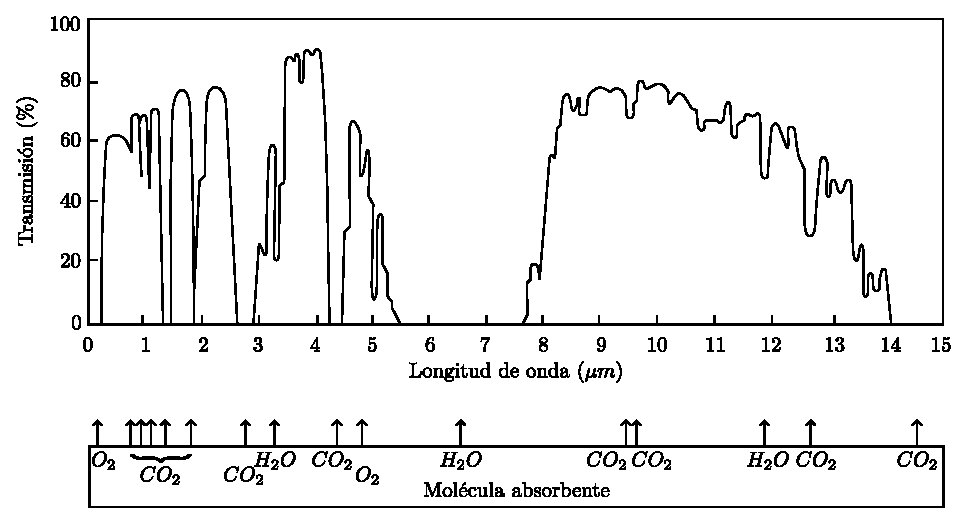
\includegraphics[width=0.8\textwidth]{atmos_window}
                \caption{Transmisión de la atmósfera.}
                \label{fig:atmos_window}
            \end{figure}



Despejando la temperatura de la ecuación \ref{eq:Wien} \cite{BlancoMDA}:
    \begin{equation}
        T_{max} = \frac{2.90\times10^{-3}\ mK}{8\mu m} = 362.5K
        \label{eq:tempmax}
    \end{equation}

    \begin{equation}
        T_{min} = \frac{2.90\times10^{-3}\ mK}{14\mu m} = 207.14K
        \label{eq:tempmin}
    \end{equation}

podemos deducir que los detectores infrarrojos que operan en la ventana de 8 - 14 $\mu m$ tienen mayor sensibilidad a la temperatura ambiente \cite{Rogalski}.

El material de fabricación y longitud de onda de operación de los detectores infrarrojos cambian de acuerdo a la aplicación en la que se desee trabajar \cite{Rogalski}.					           
     
    
    \section{Detectores Infrarrojos}
    
    Un detector infrarrojo es un dispositivo capaz de absorber parte de la energía infrarroja radiada hacia él, provocando una variación en alguna de sus propiedades eléctricas \cite{BlancoMDA}. Podemos pensar en un detector infrarrojo como un transductor, el cual convierte un tipo de señal en otra; el detector infrarrojo convierte la radiación infrarroja incidente en una señal eléctrica \cite{Vincent}.
    
    Dependiendo de la aplicación, el rango del espectro electromagnético y la temperatura en los que se desee trabajar, se debe diseñar o utilizar un detector específico que cumpla con los requerimientos, ya que cada aplicación requiere características diferentes a las demás \cite{Rogalski},\cite{BlancoMDA}.
    
    Los detectores infrarrojos se pueden clasificar en dos categorías: \textit{Detectores de fotones} y \textit{detectores térmicos}.
    
		\subsection{Detectores de fotones}
		En los detectores de fotones, la formación de pares electrón-hueco es consecuencia de la detección de radiación absorbida \cite{BlancoMDA}. En estos dispositivos, el fotón que incide sobre la superficie del material puede ser absorbido, lo que resulta en la remoción de un electrón desde la banda de valencia o desde un estado localizado dentro de la banda prohibida hasta la banda de conducción.

Generalmente, los detectores de fotones que operan a longitudes de onda de aproximadamente 3$\mu m$ requieren de un sistema de enfriamiento. Esto es necesario para prevenir la generación térmica de portadores de carga, la cual es su principal desventaja, ya que aumenta su costo y complejidad de operación. No obstante, su resolución y desempeño son bastante buenos \cite{Vincent},\cite{BlancoMDA}. 
		   
		\subsection{Detectores térmicos}
		El funcionamiento de los detectores térmicos se basa en la generación de una salida eléctrica medible como resistencia o diferencia de potencial debido al cambio de temperatura del material causado por la radiación incidente.
Estos detectores pueden funcionar a temperatura ambiente, son económicos, compactos, de bajo consumo energético y tienen una larga vida útil, pero su capacidad de detección es baja \cite{Rogalski},\cite{BlancoMDA}.
Algunos de los principales detectores térmicos infrarrojos son explicados a continuación.
		
		\subsubsection{Celda de Golay}
		La celda de Golay es un detector térmico principalmente utilizado en espectroscopía infrarroja, la celda consiste en una cámara herméticamente cerrada llena de gas y un espejo flexible. A medida que la radiación infrarroja incide, el gas se calienta y se expande, provocando que el espejo flexible se mueva. El movimiento del espejo desvía un haz de luz que incide sobre otro detector generando un cambio en su irradiancia, después esa señal es procesada \cite{Vincent},\cite{BlancoMDA}.
		\subsubsection{Bolómetros y Microbolómetros}
		Los bolómetros y microbolómetros son dispositivos que detectan la radiación infrarroja mediante el cambio en la resistencia eléctrica de un material al variar su temperatura. Conforme la resistencia absorbe calor, su temperatura aumenta y su resistencia se modifica.
Este tipo de sensores deben polarizarse con corriente o voltaje para que puedan funcionar.
Si son polarizados con corriente, el cambio de la resistencia se puede detectar y medir como un cambio de tensión, pero si se polariza con voltaje entonces se detectará como un cambio de corriente \cite{Rogalski},\cite{Vincent}.
		\subsubsection{Termopares y Termopilas}
		Los termopares y las termopilas están formados por la unión de dos conductores diferentes unidos por un extremo. Cuando la temperatura aumenta en esa unión, se genera una diferencia de potencial. Al conectar en serie varias uniones de conductores, se produce una tensión más elevada y, por lo tanto, medible \cite{Rogalski},\cite{Vincent}.
		
		\subsubsection{Detectores piroeléctricos y ferroeléctricos}
		Estos detectores pueden visualizarse como un capacitor con dos electrodos metálicos colocados perpendicularmente. Cuando un detector piroeléctrico absorbe radiación, su temperatura cambia, lo que genera una carga en el capacitor y una corriente que depende del cambio de temperatura. Si la temperatura permanece constante, la corriente será nula.

Los detectores ferroeléctricos operan bajo el mismo principio que los piroeléctricos, pero con la diferencia de que el efecto se produce mediante un campo eléctrico \cite{Rogalski}, \cite{BlancoMDA}.


En los últimos años, ha habido un creciente interés en el uso de microbolómetros para generar imágenes infrarrojas. En el ámbito médico, se han utilizado para medir la temperatura corporal \cite{Svantner2022} y, de manera innovadora, en el diagnóstico de la diabetes, mediante la captura de imágenes térmicas de la lengua \cite{WziatekKuczmik2024} o del pie \cite{Rocha2022}, permitiendo identificar variaciones térmicas que pueden indicar problemas de salud. Otra aplicación importante es en cámaras instaladas en vehículos, donde los microbolómetros se emplean para detectar personas o mascotas una vez detenido el vehículo, ayudando a prevenir accidentes ocasionados por quedar atrapados dentro \cite{Farhat2011}.


Este creciente interés se debe, en parte, a su bajo costo, peso ligero y dimensiones reducidas, que pueden ser menores a 12 $\mu$m, lo que permite una mayor cantidad de pixeles en un arreglo. Además, mientras que algunos sensores infrarrojos están limitados a resoluciones de 120$\times$84 pixeles, los microbolómetros pueden alcanzar resoluciones mucho más altas, como 1280$\times$1024 o más, obteniendo imágenes más detalladas y nítidas. Estas ventajas hacen de los microbolómetros una opción preferida en tecnologías de imágenes térmicas de alta precisión. Por este motivo, en este trabajo se desarrollará un sistema de adquisición de datos modular, que puede ser utilizado con un microbolómetro. En la siguiente tabla se presentan trabajos similares.

            \begin{table}[htbp]
                \caption{Resumen de trabajos relacionados son sistemas de lectura para detectores.}
                \begin{center}
                    \resizebox{1\linewidth}{!}{ 
                    \begin{NiceTabular}{|c|c|c|c|c|c|}
                        \CodeBefore
                        \Body
                        \hline
                        \textbf{Artículo} & \textbf{Dispositivo de implementación} & \textbf{Tecnología de detección} & \textbf{Sistema configurable} & \textbf{Interfaz gráfica} & \textbf{Arreglo máximo de detectores} \\
                        \hline
                        \multirow{2}{*}{\cite{Farhat2011}} & \multirow{2}{*}{TSK3000 Microcontrolador incluido en FPGA Altera company} & \multirow{2}{*}{Microbolómetro no refrigerado de Silicio-amorfo (a-Si)} & \multirow{2}{*}{No} & \multirow{2}{*}{Integrada} & \multirow{2}{*}{168x120} \\&  &  &  &  &  \\
                        \hline
                        \multirow{2}{*}{\cite{Sosnowski2010}} & \multirow{2}{*}{FPGA EPC2C35F672 de Altera company} & \multirow{2}{*}{UL 03 04 (comercial) Microbolómetro de Silicio-amorfo (a-Si)} & \multirow{2}{*}{No} & \multirow{2}{*}{No} & \multirow{2}{*}{384x288} \\&  &  &  &  &  \\
                        \hline
                        \multirow{2}{*}{\cite{Forsberg2015}} & \multirow{2}{*}{FPGA EPC3C40 de Altera company} & \multirow{2}{*}{Microbolómetro con pozo cuántico de Silicio (Si), Silicio-germanio (SiGe)} & \multirow{2}{*}{No} & \multirow{2}{*}{Sí} & \multirow{2}{*}{384x288} \\&  &  &  &  &  \\
                        \hline
                        \multirow{2}{*}{\cite{Vybornov2020}} & \multirow{2}{*}{Microcontrolador Cortex M3 STM32F103} & \multirow{2}{*}{Bolómetro en sustrato de Óxido de aluminio (Al2O3), Silicio (Si)} & \multirow{2}{*}{No} & \multirow{2}{*}{No} & \multirow{2}{*}{1x1} \\&  &  &  &  &  \\
                        \hline
                        \multirow{2}{*}{\cite{Xie2016}} & \multirow{2}{*}{FPGA Cyclone IV EP4CE55 de Altera company} & \multirow{2}{*}{GWR1020 IRFPA de Óxido de vanadio (VOx)} & \multirow{2}{*}{No} & \multirow{2}{*}{No} & \multirow{2}{*}{384x288} \\&  &  &  &  &  \\
                        \hline
                        \multirow{2}{*}{\cite{Feng2020}} & \multirow{2}{*}{DSP TMS320DM6467} & \multirow{2}{*}{Microbolómetro UL04371 (comercial)} & \multirow{2}{*}{No} & \multirow{2}{*}{No} & \multirow{2}{*}{160x120} \\&  &  &  &  &  \\
                        \hline
                        \multirow{2}{*}{\cite{Bayareh2018}} & \multirow{2}{*}{Raspberry Pi 2} & \multirow{2}{*}{Lepton FLIR 2.5 (comercial): Microbolómetro de VOx no refrigerado} & \multirow{2}{*}{No} & \multirow{2}{*}{Si} & \multirow{2}{*}{80x60} \\&  &  &  &  &  \\
                        \hline
                        \multirow{2}{*}{\cite{LeneroBardallo2022}} & \multirow{2}{*}{Raspberry Pi 3 B+} & \multirow{2}{*}{Lepton FLIR (comercial): Microbolómetro de VOx no refrigerado} & \multirow{2}{*}{No} & \multirow{2}{*}{No} & \multirow{2}{*}{160x120} \\&  &  &  &  &  \\
                        \hline
                        \multirow{2}{*}{\cite{Rocha2022}} & \multirow{2}{*}{Raspberry Pi} & \multirow{2}{*}{Lepton FLIR 2.5 (comercial): Microbolómetro de VOx no refrigerado} & \multirow{2}{*}{No} & \multirow{2}{*}{No} & \multirow{2}{*}{80x60} \\&  &  &  &  &  \\
                        \hline
                        \multirow{2}{*}{\cite{Javaid2020}} & \multirow{2}{*}{DROIC} & \multirow{2}{*}{Infrared pixel array} & \multirow{2}{*}{Si} & \multirow{2}{*}{Si} & \multirow{2}{*}{1024x1024} \\&  &  &  &  &  \\
                        \hline
                    \end{NiceTabular}
                    }
                \label{tab:Div_IR}
                \end{center}
            \end{table}	 					          
		
    \section{Objetivos}
	
		\subsection{Objetivo general}
			\begin{itemize}
				\item Diseño de un sistema de adquisición de datos basado en FPGA para la medición de una matriz de pixeles de un microbolómetro.
			\end{itemize}
		
		\subsection{Objetivos específicos}
			\begin{itemize}
                \item Analizar las propiedades físicas y características de los microbolómetros, así como su funcionamiento y sus diferentes circuitos de lectura con el fin de fundamentar las decisiones en el diseño del sistema.
                \item Estudiar las máquinas de estado finito (FSM) de tipo Moore y Mealy, los tipos de codificación en Verilog y las técnicas de diseño, con el fin de aplicar este conocimiento en la implementación y optimización del sistema de adquisición y procesamiento de datos.
                \item Diseñar un firmware en el lenguaje Verilog para implementar los protocolos de comunicación SPI y UART reconfigurables y robustos, que permitan adaptabilidad y confiabilidad en aplicaciones de adquisición de datos y control.
                \item Seleccionar los convertidores analógico-digital (ADC) y digital-analógico (DAC) más adecuados para el sistema de adquisición de datos y probarlos utilizando el firmware previamente diseñado.
                \item Diseñar una PCB con una matriz de 8x8 fototransistores que funcione como banco de prueba para validar el funcionamiento del sistema de adquisición de datos.
                \item Integrar los convertidores ADC y DAC, multiplexores, y la matriz de fototransistores en un sistema unificado para realizar pruebas y validar su capacidad de adquirir y procesar imágenes de manera eficiente.
			\end{itemize}

	\chapter{Microbolómetros y descripción de especificaciones}

    \section{Propiedades}
    En esta sección se definirán algunas propiedades importantes que son utilizadas para caracterizar el desempeño de microbolómetros.
        \subsection{Responsividad}
        La responsividad ($R$) se refiere a la capacidad que tiene un detector de convertir radiación incidente en una señal eléctrica
        \begin{equation}
        R = \frac{se\tilde{n}al\ de\ salida}{radiaci\acute{o}n\ de\ entrada}
        \label{eq:Responsividad_0}
        \end{equation}
        
        Para los microbolómetros, generalmente la radiación de entrada se define en términos de flujo radiante ($\Phi_{S}$), el cual es el producto de la irradiancia ($E$) por el área del detector ($A_{d}$) y la señal de salida  puede ser voltaje ($V_{S}$) o corriente ($I_{S}$).
        \begin{equation}
        R = \frac{S}{\Phi_{S}}
        \label{eq:Responsividad}
        \end{equation}
        
        La responsividad de voltaje $R_{V}$ se define como:
        \begin{equation}
        R_{V} = \frac{V_{S}}{EA_{d}}\phantom{abc} [V/W]
        \label{eq:Responsividad-voltaje}
        \end{equation}
        
        La responsividad de corriente es:
        \begin{equation}
        R_{I} = \frac{I_{S}}{EA_{d}}\phantom{abc} [A/W]
        \label{eq:Responsividad-corriente}
        \end{equation}
        
        La responsividad es un parámetro crucial para un detector, ayuda a anticipar la sensibilidad del circuito de medición necesario para observar la salida esperada o a decidir el nivel de ganancia del amplificador requerido para amplificar la señal adecuadamente.
        
        \subsection{Diferencia de temperatura equivalente al ruido}
        La diferencia de temperatura equivalente al ruido (Noise Equivalent Temperature Difference - $NETD$), indica el cambio mínimo de temperatura que un microbolómetro puede detectar, reflejando su capacidad para distinguir pequeñas diferencias en la radiación térmica. Un valor de $NETD$ más bajo significa mayor sensibilidad térmica.
        El $NETD$ se calcula con la siguiente fórmula:
        \begin{equation}
        NETD = \frac{(4(f/D)^{2} + 1)V_{N}}{\tau_{0}AR_{V}(\Delta P/\Delta T)_{\lambda_{1} - \lambda_{2}}}\phantom{abc} [K]
        \label{eq:NETD}
        \end{equation}        
        Donde:
        
        $f$
        
        $D$
        
        $V_{N}$
        
        $\tau_{0}$
        
        $A$
        
        $R_{V}$
        
        \subsection{Detectividad}
        \subsection{Conductancia térmica}
        \subsection{Capacitancia térmica}
        \subsection{Coeficiente de temperatura de la resistencia}


\section{Diseño y fabricación}

\section{Circuitos de lectura para un microbolómetro}
	\chapter{Sistema de adquisición de datos DAQ}

  \section{Visión general de la comunicación serial}

    Con frecuencia, un sistema necesita comunicarse con otro que no reside en el mismo dispositivo. Para reducir el número de pines de I/O y el cableado externo, los dos sistemas pueden transferir datos a través de una única línea serial, bit a bit. El sistema transmisor realiza la conversión de paralelo a serie y, a continuación, envía los datos serie a través de una única línea. El sistema receptor realiza la conversión serie a paralelo y restaura los datos paralelos originales.

    La comunicación serial puede utilizarse tanto para transferir datos a alta velocidad como a baja velocidad. En una interfaz de alta velocidad, como USB y gigabit Ethernet, la velocidad de transmisión de datos puede alcanzar varios cientos de millones de bits por segundo o más. 

    En una interfaz de baja velocidad, la velocidad de transmisión de datos oscila entre varios miles y varios cientos de miles de bits por segundo. Es adecuada para la mayoría de los periféricos de I/O generales y para tareas de adquisición y control de datos. Dado que la velocidad de datos es mucho más lenta que la velocidad de reloj de una FPGA, estos esquemas pueden ser realizados por los elementos lógicos genéricos de una FPGA. A continuación se discuten los esquemas UART y SPI.

	\section{Controlador UART}

    La comunicación serial utiliza una única línea de datos para intercambiar información entre dos sistemas. El sistema transmisor convierte los datos paralelos en un flujo serie y el sistema receptor vuelve a ensamblar los datos serie en su formato paralelo original. El esquema más utilizado es el UART, (Universal Asynchronous Receiver and Transmitter) o receptor y transmisor asíncrono universal en español.

    \subsection{Visión general}

    Un controlador UART básico incluye un transmisor y un receptor. El transmisor es un registro de corrimiento especial que carga datos en paralelo y luego los desplaza bit a bit a una velocidad específica. El receptor, por su parte, desplaza los datos bit a bit y los vuelve a ensamblar. La línea serial es 1 cuando está inactiva. La transmisión comienza con un bit de inicio, que es 0, seguido de bits de datos y un bit de paridad opcional, y termina con bits de parada, que son 1. El número de bits de datos puede ser 6, 7 u 8. El bit de paridad opcional se utiliza para la detección de errores. Para paridad impar, se pone a 0 cuando los bits de datos tienen un número impar de 1's. Para paridad par, se pone a 0 cuando los bits de datos tienen un número par de 1's. El número de bits de parada puede ser 1, 1,5 ó 2. En la Figura \ref{fig:uart_transmission} se muestra la transmisión con ocho bits de datos, sin paridad y un bit de parada. Observe que el LSB de la palabra de datos se transmite primero.

    \begin{figure}[hbtp]
      \centering
      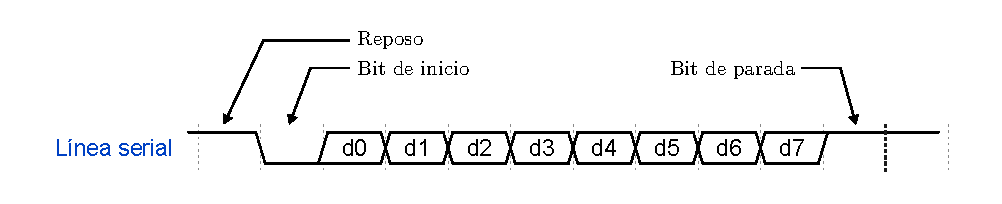
\includegraphics[width=0.95\textwidth]{uart_transmission}
      \caption{Diagrama de la transmisión de un byte serial con UART.}
      \label{fig:uart_transmission}
    \end{figure}

    A través de la línea serial no se transmite información de reloj. Antes de iniciar la transmisión, el transmisor y el receptor deben acordar de antemano una serie de parámetros, que incluyen la velocidad en baudios (es decir, el número de bits por segundo), el número de bits de datos y bits de parada, y el uso del bit de paridad. Con los parámetros predeterminados, el receptor utiliza un esquema de sobremuestreo para recuperar los bits de datos. Las velocidades en baudios más utilizadas son 9,600 y 19,200 baudios.

    \subsection{Procedimiento de sobremuestreo}

    La velocidad de muestreo más utilizada es 16 veces la velocidad en baudios, lo que significa que cada bit serie se muestrea 16 veces. Para un enlace de comunicación con N bits de datos y M bits de parada, el esquema de sobremuestreo funciona de la siguiente manera:
    
    \begin{enumerate}
      \item Espera hasta que la señal entrante se convierta en 0, el comienzo del bit de inicio, y luego comienza a contar los pulsos de muestreo.
      \item Cuando el contador llegue a 7, la señal entrante alcanzará el punto medio del bit de inicio. Limpia el contador a 0 y reinícialo.
      \item Cuando el contador llegue a 15, la señal entrante habrá avanzado un bit y alcanzará el punto medio del primer bit de datos. Obtén su valor, desplázalo a un registro y reinicia el contador.
      \item Repite el paso 3 N–1 veces más para obtener los bits de datos restantes.
      \item Si se utiliza el bit de paridad opcional, repite el paso 3 una vez para obtener el bit de paridad.
      \item Repite el paso 3 M veces más para obtener los bits de parada.
    \end{enumerate}

    El esquema de sobremuestreo realiza básicamente la función de una señal de reloj. En lugar de utilizar el flanco ascendente para indicar cuándo es válida la señal de entrada, utiliza los pulsos de muestreo para estimar el punto medio de cada bit. Aunque el receptor no tiene información sobre el momento exacto de inicio del bit, la estimación puede estar desviada como máximo en $1/16$. Las siguientes recuperaciones de bits de datos también se desvían como máximo de $1/16$ del punto medio. Debido al sobremuestreo, la velocidad en baudios sólo puede ser una pequeña fracción de la velocidad de reloj del sistema, por lo que este esquema no es apropiado para una velocidad de datos alta.


    \subsection{Diseño conceptual}

      El diagrama de alto nivel de un sistema UART se muestra en la Figura \ref{fig:uart_diagram}. Consiste en tres componentes principales. El generador de la tasa de baudios genera una señal de sobremuestreo. El receptor realiza la conversión de serie a paralelo y el transmisor realiza la conversión de paralelo a serie.

    \begin{figure}[h!]
      \centering
      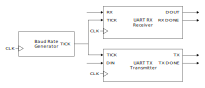
\includegraphics[width=0.8\textwidth]{uart_diagram}
      \caption{Diagrama de bloques de una controlador UART completo.}
      \label{fig:uart_diagram}
    \end{figure}

    \subsection{Generador de la tasa de baudios}

    El generador de la tasa de baudios genera una señal de muestreo cuya frecuencia es exactamente 16 veces la tasa de baudios designada para el UART. Para evitar la creación de un nuevo dominio de reloj y violar el principio de diseño síncrono, la señal de muestreo debe funcionar como pulsos de habilitación en lugar de la señal de reloj para el receptor UART.

    El generador de la tasa de baudios es un contador programable y el código HDL se muestra en el Código \ref{cod:baud_gen}. El código es un contador mod$-m$ parametrizado que se reinicia cada vez que el contador llega a un valor determinado. Por ejemplo para una tasa de 19,200 baudios, la tasa de muestreo tiene que ser de 307,200 (es decir, 19,200 $\times$ 16) pulsos por segundo. Dada una frecuencia del reloj de sistema de 50 MHz, el generador de la tasa de baudios necesita un contador mod-163, $\left( \frac{50 \times 10^{6}}{19200 \times 16} \right)$, en el cual se genera un pulso de ciclo de reloj cada 163 ciclos de reloj del sistema.

    \subsection{Receptor UART}

    \subsection{Transmisor UART}

	\section{Controlador SPI}

    El estándar SPI (Serial Peripheral Interface) o Interfaz Periférica Serial en español, es un protocolo de transferencia de datos en serie desarrollado originalmente por Motorola a principios de los 80. El bus SPI se compone de tres líneas, dos de ellas para transmitir y recibir datos en serie, y una para la señal de reloj. Se pueden conectar al bus un dispositivo maestro y varios dispositivos esclavos. El maestro genera la señal de reloj e inicia la transferencia de datos. El estándar SPI se utiliza ampliamente en sistemas embebidos para conectar módulos periféricos. \cite{Chu2018}, \cite{Chu2008}

    \subsection{Visión general}

    El estándar SPI especifica el protocolo que intercambia datos entre dos dispositivos a través de líneas seriales. En lugar de utilizar el esquema de sobremuestreo de UART, la interfaz SPI incluye una tercera línea para controlar el desplazamiento y el muestreo de los datos seriales. Las actividades se realizan en el flanco de transición de esta señal. Su función es similar a la señal de reloj de un sistema síncrono, por lo que esta línea se denomina reloj SPI.

    A diferencia de la configuración UART, en la que dos sistemas son simétricos y ambos pueden iniciar una transmisión, el estándar SPI utiliza una configuración maestro-esclavo. El maestro controla el funcionamiento general y genera la señal de reloj SPI. Sólo el maestro puede iniciar una transferencia de datos.

    A pesar de su nombre, el reloj SPI no es un reloj de sistema real y no debe utilizarse para controlar ningún registro directamente. La velocidad del reloj del sistema del controlador SPI es mucho más rápida que la velocidad del reloj SPI. Desde el punto de vista del controlador SPI, el reloj SPI es sólo otra señal de control.

    \subsection{Arquitectura del controlador}

    El diagrama conceptual de un bus SPI con dos dispositivos se muestra en la Figura \ref{fig:spi_diagram}. Tanto el maestro como el esclavo tienen un registro de desplazamiento (shift register) en su interior. Los dos registros de desplazamiento están conectados como un anillo a través de las líneas MOSI (para Master-Out-Slave-In) y MISO (para Master-In-Slave-Out) y su funcionamiento está coordinado por la misma señal de reloj SPI, SCLK. 

    Las señales MOSI y MISO son algo así como la señal de transmisión (TX) y la señal de recepción (RX) del UART. Suponemos que ambos registros tienen ocho bits de ancho y que la transferencia de datos se realiza byte a byte. Al principio de la operación, tanto el maestro como el esclavo cargan datos en los registros. Durante la transferencia de datos, los datos de ambos registros se desplazan un bit a la derecha en cada ciclo SCLK. Tras ocho ciclos SCLK, se han desplazado ocho bits de datos y el maestro y el esclavo han intercambiado los valores de los registros. A continuación, el maestro y el esclavo pueden procesar los datos recibidos. Esta operación puede interpretarse como que el maestro escribe datos en el esclavo y los lee simultáneamente, lo que se conoce como operación full-duplex.

    \begin{figure}[hbtp]
        \centering
        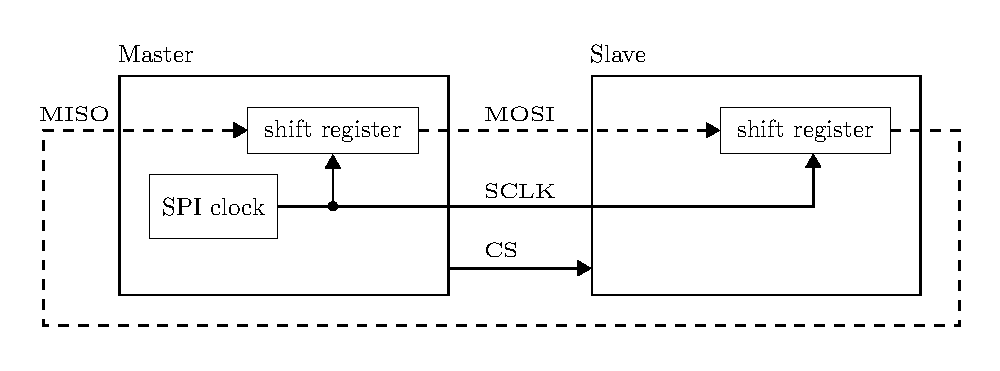
\includegraphics[width=0.8\textwidth]{spi_diagram}
        \caption{Diagrama conceptual del bus SPI.}
        \label{fig:spi_diagram}
    \end{figure}    

    Además de las líneas MOSI, MISO y SCLK, un dispositivo esclavo también puede tener una entrada de selección de chip activa en bajo, SS (para Slave Select). En otros casos también puede tener el nombre de  CS (para Chip-Select). Se puede utilizar para que el maestro seleccione el dispositivo esclavo deseado si hay varios dispositivos esclavos en el bus. Muchos dispositivos SPI también utilizan CS para ciertas funcionalidades de control y no se puede omitir, incluso en una configuración de un solo esclavo.

    \subsection{Configuración de múltiples dispositivos}

    El estándar SPI admite una configuración múltiple-esclavo, en la que un dispositivo maestro puede controlar más de un dispositivo esclavo. Existen dos esquemas básicos, que son la configuración en paralelo y la configuración en cadena.

    La configuración en paralelo utiliza una línea CS dedicada para cada dispositivo esclavo, como se muestra en la Figura \ref{fig:spi_parallel}. Una línea CS funciona como señal de selección de chip y el maestro puede seleccionar el dispositivo deseado activando la línea correspondiente. Esta configuración puede acomodar un maestro y dispositivos esclavos independientes. Dado que las líneas MISO de los esclavos están unidas, la línea MISO debe ser controlada por un buffer de tres estados y su salida debe estar en un estado de alta impedancia cuando el dispositivo esclavo no está seleccionado. 

    \begin{figure}[hbtp]
      \centering
      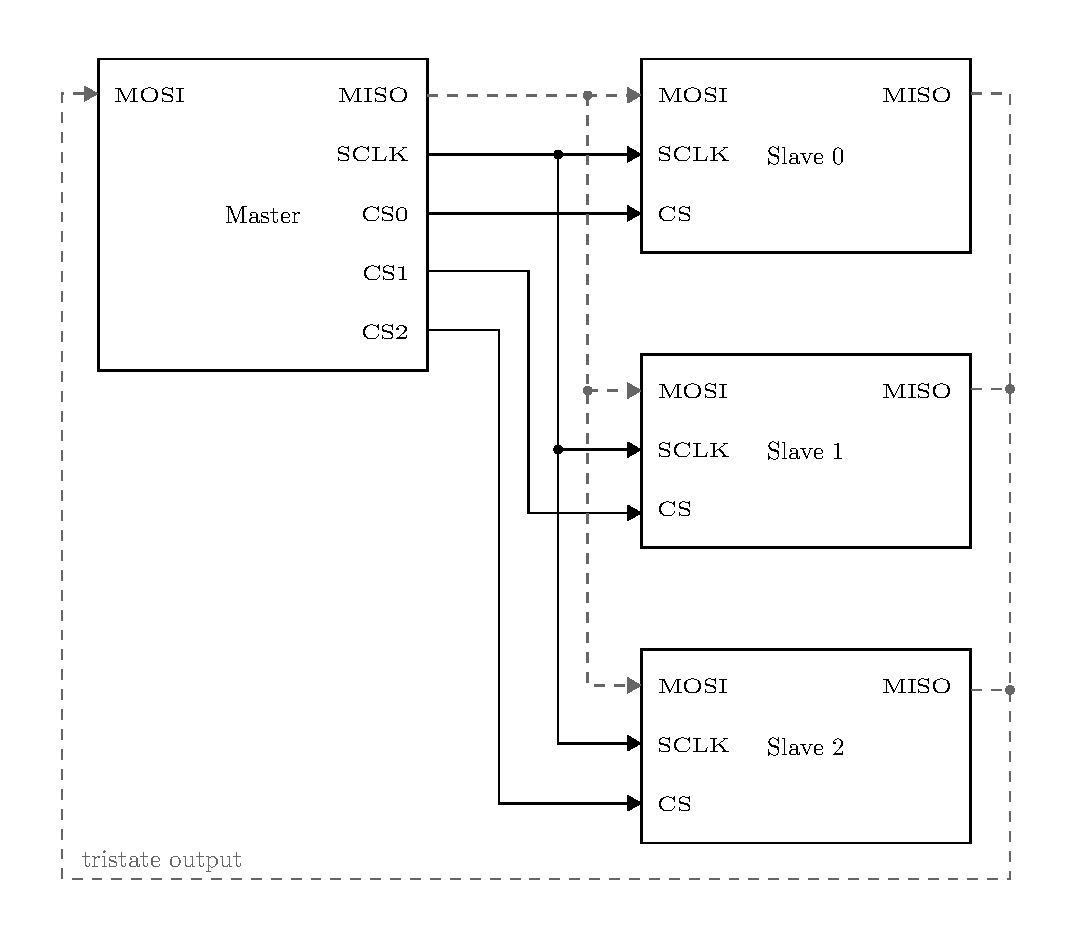
\includegraphics[width=0.8\textwidth]{spi_parallel}
      \caption{Configuración en paralelo de bus SPI.}
      \label{fig:spi_parallel}
    \end{figure}    

    La configuración en cadena conecta las líneas MOSI y MISO en una cadena en cascada, como se muestra en la Figura \ref{fig:spi_chain}. Se utiliza una única línea CS para controlar todos los dispositivos esclavos. Conceptualmente, la cadena forma un gran registro de desplazamiento y los datos se transfieren en serie de dispositivo a dispositivo. Los dispositivos de esta configuración deben ser cooperativos y seguir el mismo protocolo para transmitir, insertar y extraer bytes de datos.

    \begin{figure}[hbtp]
      \centering
      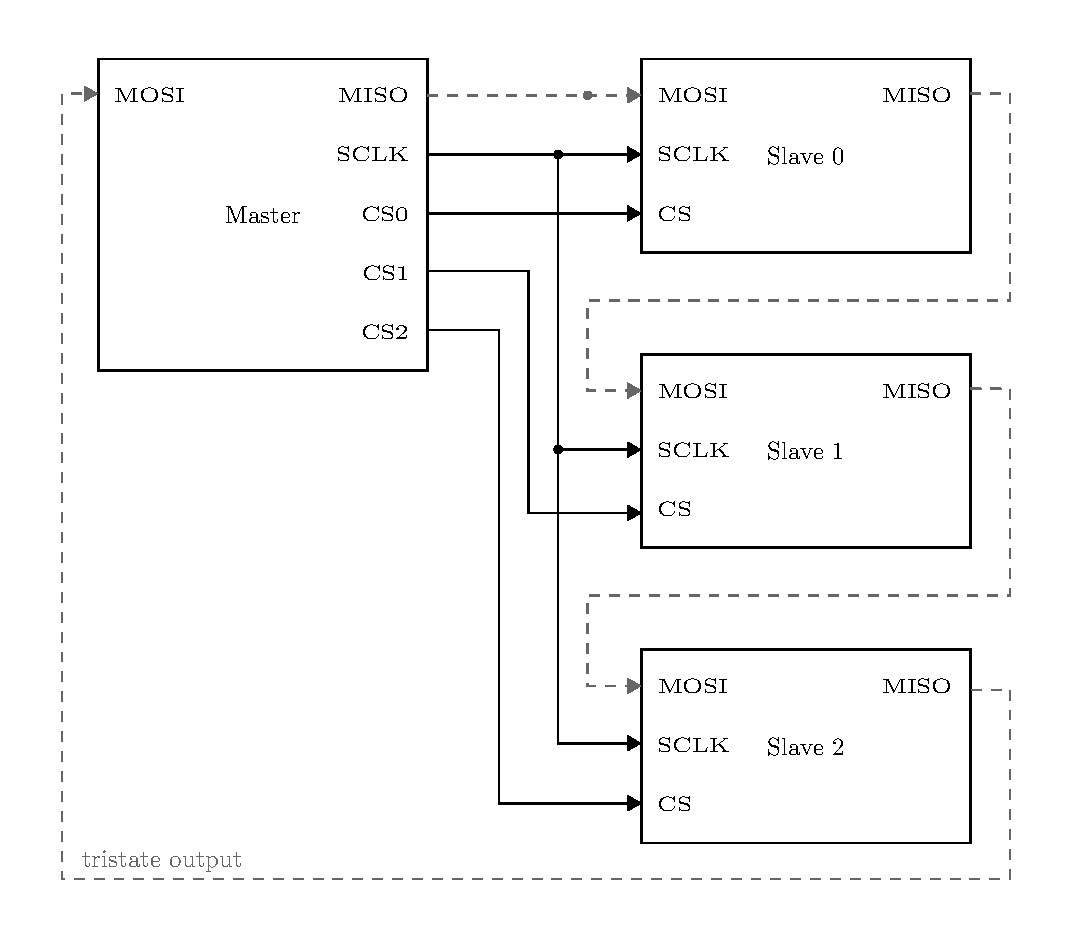
\includegraphics[width=0.8\textwidth]{spi_chain}
      \caption{Configuración en cadena de bus SPI.}
      \label{fig:spi_chain}
    \end{figure}    


    \subsection{Sincronización del controlador}

    El bus SPI utiliza los flancos del reloj SPI (SCLK) para controlar y sincronizar la transferencia de bits de los datos. Para aclarar la explicación, se definen dos actividades durante una transferencia de bits: enviar (es decir, desplazar) un nuevo bit a la línea de datos y muestrear (es decir, capturar) un bit de la línea de datos. El envío y el muestreo se completan en el mismo ciclo de reloj SPI, pero ocurren en flancos de reloj opuestos.
    En la Figura \ref{fig:spi_timing_diagram} se muestra un diagrama de tiempos representativo. Inicialmente, el bus está inactivo y la línea SCLK está en 0. En $t_{0}$, el maestro activa CS y el esclavo designado coloca el primer bit de datos (bit 7) en la línea MISO. En $t_{1}$, el maestro inicia el reloj SPI y envía el bit b7 en la línea MOSI.
Dado que la primera mitad del periodo del reloj SPI es 0, el valor en SCLK permanece sin cambios. El tiempo que transcurre entre $t_{0}$ y $t_{1}$ puede ser muy pequeño o incluso cero. En $t_{2}$, el maestro sube el reloj SPI y avanza a la segunda mitad del periodo del reloj. En el flanco de transición de 0 a 1, el maestro muestrea los datos en MISO y el esclavo los datos en MOSI. 
     En $t_{3}$, se completa el primer ciclo de reloj SPI. El maestro comienza el segundo periodo de reloj SPI y baja SCLK. Tanto el maestro como el esclavo envían nuevos bits a la línea de datos. En $t_{4}$, el maestro vuelve a subir SCLK y tanto el maestro como el esclavo muestrean los nuevos bits de datos. Las actividades de transmisión y muestreo se repiten hasta que se transfieren ocho bits de datos. Los últimos datos se muestrean en $t_{5}$ y SCLK vuelve a 0 en $t_{6}$. En $t_{7}$, el maestro desactiva CS. Cabe destacar que todos los muestreos se realizan en los flancos ascendentes de SCLK y todas las transmisiones (excepto la inicial) se realizan en los flancos descendentes de SCLK.

    \begin{figure}[hbtp]
      \centering
      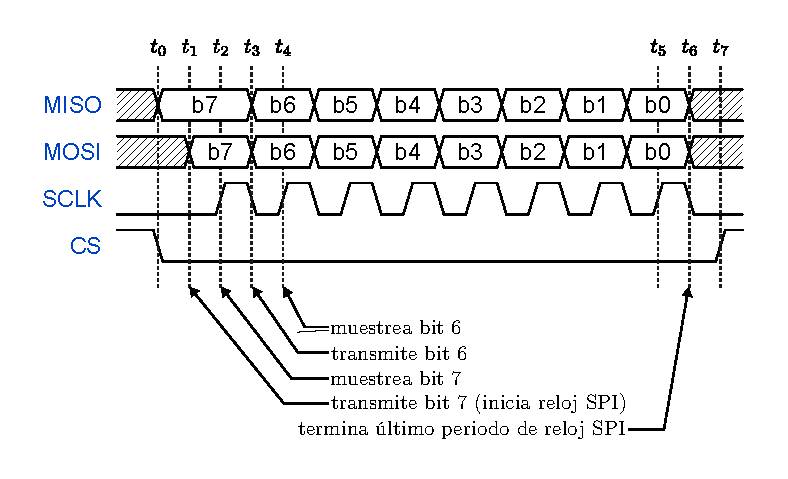
\includegraphics[width=0.8\textwidth]{spi_timing_diagram}
      \caption{Diagrama de tiempos representativo de una transferencia de datos SPI.}
      \label{fig:spi_timing_diagram}
    \end{figure}

    \subsection{Modos de operación}

    El modo de operación del SPI define las relaciones entre los flancos del reloj SPI y las actividades de envío y muestreo en las líneas de datos. Hay cuatro modos. Los modos dependen de dos parámetros, que son la polaridad del reloj (abreviado como CPOL, Clock Polarity) y la fase del reloj (abreviado como CPHA, Clock Phase). La polaridad del reloj se define como el valor de SCLK cuando está en reposo, que puede ser 0 o 1. La fase del reloj es más difícil de definir. Una interpretación es si un flanco del reloj se utiliza para enviar el primer bit de datos. Si CPHA es 1, el maestro conduce el bit en el primer flanco de transición. Si CPHA es 0, el maestro envía el bit en el flanco de transición cero, inmediatamente cuando CS se activa (lo que significa que no hay flanco o no en el primer flanco).

    Basándose en los dos parámetros, los modos de operación del SPI se definen como sigue:

    \begin{table}[h!]
      \caption{Modos de operación del SPI.}
      \begin{center}
      \resizebox{\textwidth}{!}{
        \begin{NiceTabular}{|c|c|c|c|c|}
          \hline
          \textbf{Modos SPI} & \textbf{Clock polarity} & \textbf{Clock phase } & \textbf{Los datos de desplazan en } & \textbf{Los datos se muestrean en }\\
                             & \textbf{(CPOL)}         & \textbf{(CPHA)}       &                                     & \\
          \hline
          0 & 0 & 0 & bajada SCLK, y cuando CS se activa & subida SCLK \\
          1 & 0 & 1 & subida SCLK & bajada SCLK \\
          2 & 1 & 0 & subida SCLK, y cuando CS se activa & bajada SCLK \\
          3 & 1 & 1 & bajada SCLK & subida SCLK \\
          \hline
        \end{NiceTabular}
      }
      \label{tab:spi_modes}
      \end{center}
    \end{table}

    Observe que el diagrama de tiempos de la Figura \ref{fig:spi_timing_diagram} corresponde al modo 0, ya que SCLK es 0 cuando está inactivo y el primer bit no es transmitido por el primer flanco de transición.

    El diagrama de tiempo de los cuatro modos se muestra en la Figura \ref{fig:spi_timing_diagram_modes}. El modo 0 es el modo más comúnmente utilizado. En este modo, el valor en reposo es 0 y el ciclo del reloj comienza con 0. Dado que el valor en reposo y el valor inicial del reloj son los mismos, el primer bit de datos se transmite antes del primer flanco de transición. En el modo 1, el valor en reposo también es 0, pero el ciclo del reloj comienza con 1. El valor inicial de 1 lleva a una transición de 0 a 1, por lo tanto, el primer bit se transmite en el primer flanco. Es importante notar que en estos dos modos, el período del reloj y el tiempo de inicio son los mismos, pero sus valores están fuera de fase.

    \begin{figure}[!h]
      \centering
      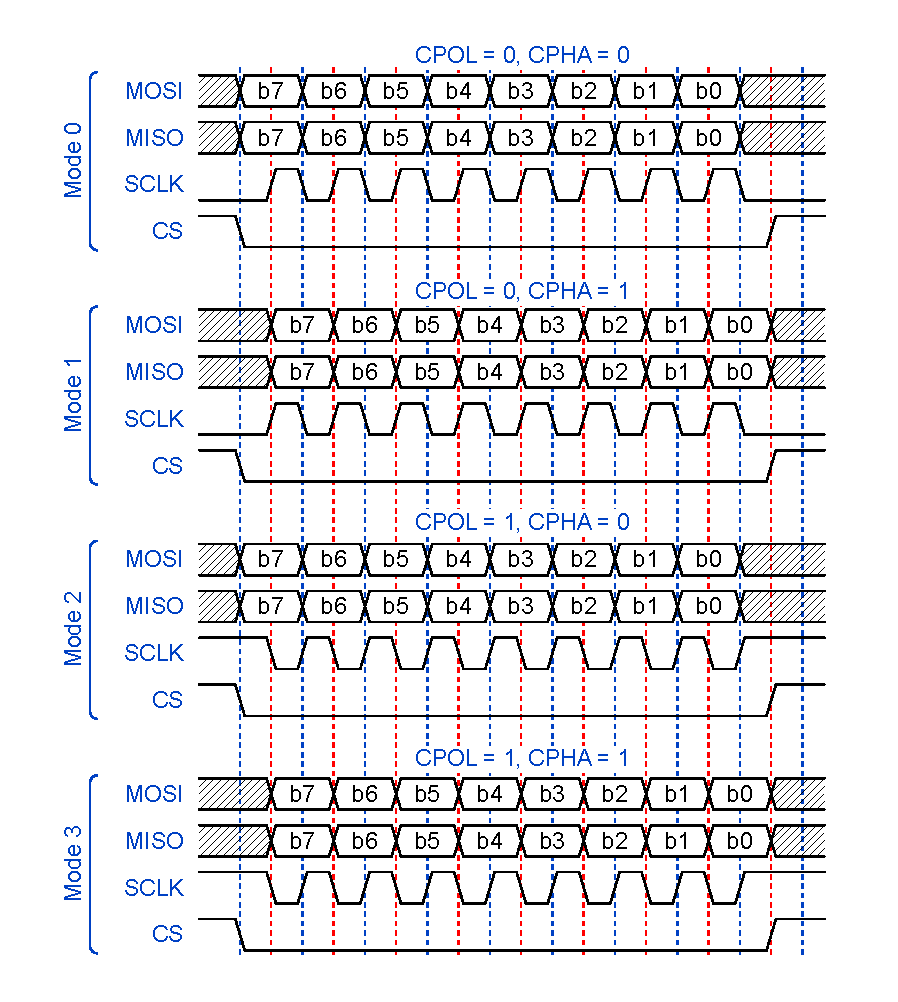
\includegraphics[width=0.85\textwidth]{spi_timing_diagram_modes}
      \caption{Diagrama de tiempos de los diferentes modos SPI.}
      \label{fig:spi_timing_diagram_modes}
    \end{figure}

    El valor en reposo de SCLK en los modos 2 y 3 es 1. La forma de onda de SCLK en el modo 2 es exactamente opuesta a la del modo 0, y la forma de onda en el modo 3 es exactamente opuesta a la del modo 1. Nuevamente, es importante destacar que el período del reloj y el tiempo de inicio son los mismos para todos los modos.

    \subsection{Aspectos indefinidos}

    La interfaz SPI fue desarrollada por Motorola y se ha convertido en un estándar de facto. No existe un organismo rector u organización que supervise este estándar. Varios aspectos importantes no están definidos en el estándar.

    El primer aspecto es el uso de la señal CS. La señal CS actúa principalmente como una señal de habilitación o selección de chip. Un dispositivo esclavo se desactiva si su señal CS no está activa. En muchos dispositivos, la señal CS también funciona como una señal de control. El intercambio de datos se realiza transacción por transacción:

    \begin{itemize}
      \item El maestro activa CS.
      \item El maestro y el esclavo seleccionado transfieren bits de datos.
      \item El maestro desactiva CS.
    \end{itemize}

    Una transacción se muestra en la Figura \ref{fig:spi_timing_diagram_aspects}. Las transiciones causadas por la activación y desactivación de CS se utilizan para activar ciertas acciones, como enviar un bit o capturar datos en paralelo, en el dispositivo esclavo. Esto implica que CS debe estar conectado al maestro, incluso si solo hay un dispositivo esclavo; es decir, simplemente conectarlo a 0 no funcionará. El estándar SPI no define explícitamente el papel de la señal CS ni el protocolo en la transacción. Además, los requisitos de temporización como el tiempo de preparación de CS ($\text{t}_{\text{SS\_SETUP}}$), que es el intervalo entre la activación de CS y el inicio del reloj, el tiempo de retención de CS ($\text{t}_{\text{SS\_HOLD}}$), que es el intervalo entre la desactivación de CS y la terminación del reloj, y el tiempo de cambio entre dos transacciones ($\text{t}_{\text{SS\_TURN}}$) no esta especificado.

    \begin{figure}[!h]
      \centering
      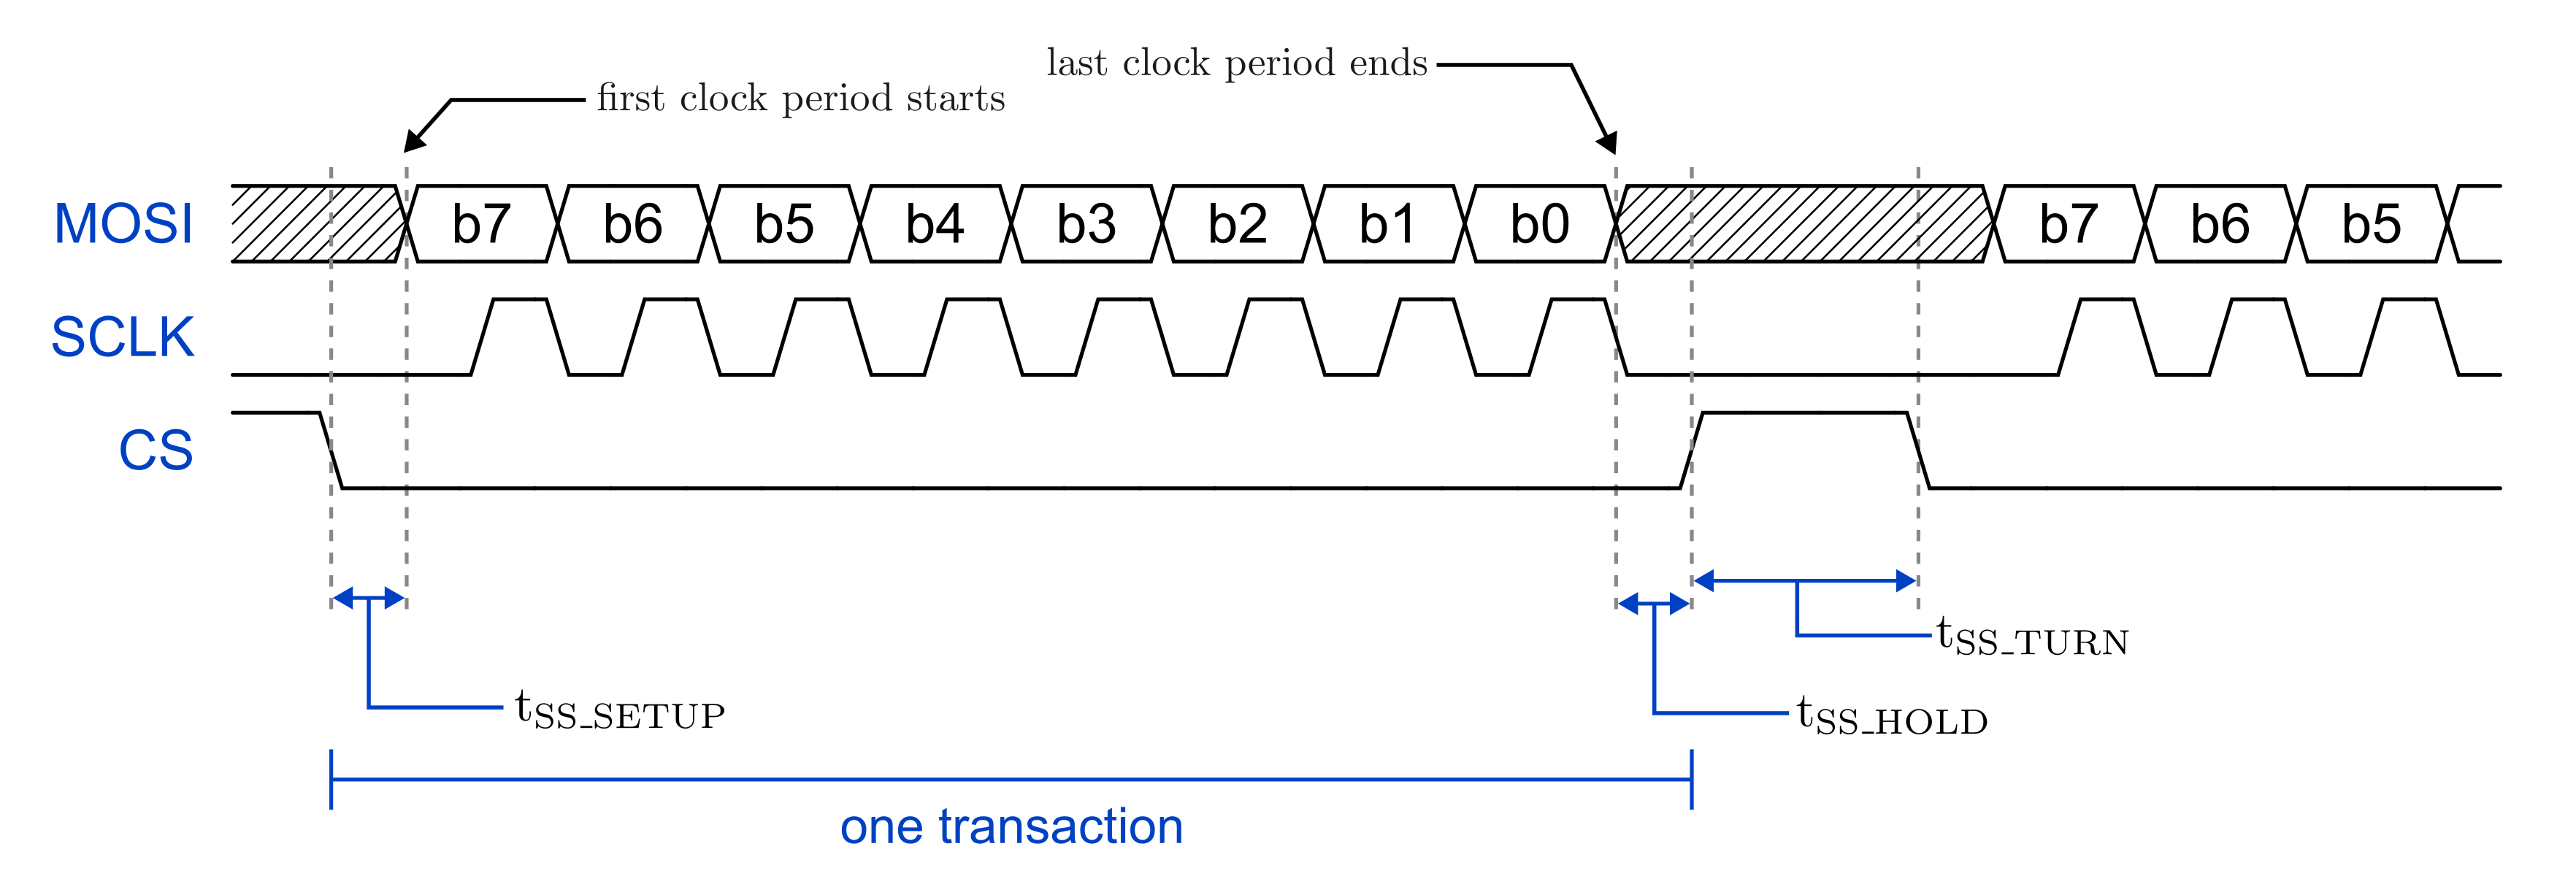
\includegraphics[width=0.95\textwidth]{spi_timing_diagram_aspects}
      \caption{Diagrama de tiempos con aspectos indefinidos, SPI modo 0.}
      \label{fig:spi_timing_diagram_aspects}
    \end{figure}

    El segundo aspecto indefinido es el número de bits en un intercambio de datos. En la Figura \ref{fig:spi_timing_diagram} se transfieren ocho bits. Sin embargo, el estándar SPI no especifica el número de bits transferidos en una transacción.

    Finalmente, el estándar SPI no especifica el orden de bits de la transmisión, es decir, si se transfiere primero el bit mas significactivo (MSB) o el bit menos significativo (LSB) de un byte de datos o de una palabra de datos. El MSB se utiliza comúnmente, pero no está garantizado.

    Debido a estos aspectos indefinidos, debemos consultar la hoja de datos del dispositivo y adaptar el acceso para cada dispositivo. Esto suele hacerlo el controlador de software y el programa de aplicación.

	\section{Digital-To-Analog Converters}

	\section{Analog-To-Digital Converters}

  Los convertidores analógico-digitales (ADC) traducen las magnitudes analógicas, características de la mayoría de los fenómenos del «mundo real», a lenguaje digital, utilizado en el tratamiento de la información, la informática, la transmisión de datos y los sistemas de control. Los convertidores de digital a analógico (DAC) se utilizan para transformar los datos transmitidos o almacenados, o los resultados del procesamiento digital, de nuevo en variables del «mundo real» para su control, visualización de información o procesamiento analógico posterior.
	

	\chapter{Implementación de TRNG híbrido}

    En este capítulo se describen los pasos para diseñar un mapa caótico y un ERO-TRNG en FPGA para generar bits aleatorios que servirán como semilla a las condiciones del mapa. Se analiza cómo seleccionar el tamaño de palabra de punto fijo utilizando un simulador en C, cómo mejorar el uso de recursos con multiplicadores de una constante y cómo seleccionar el rango valido de la semilla utilizando el dominio de atracción del mapa caótico.

   
	\chapter{Mediciones y resultados}
En este capítulo se presentan los resultados del diseño del protocolo SPI utilizado para controlar los convertidores D/A y A/D, así como los resultados obtenidos de la caracterización de resistencias, multiplexores y fotorresistencia. Además, se muestran las imágenes generadas por la matriz de fototransistores, evidenciando el correcto funcionamiento del sistema de adquisición de datos implementado y de la PCB diseñada.


\section{Resultados de protocolo SPI}
Para probar el funcionamiento del diseño del protocolo SPI, se utilizó un potenciómetro al que se varió la resistencia, conectado a un canal del convertidor A/D. Para evaluar el convertidor D/A, se asignó un valor de voltaje en formato binario. Las señales generadas por los módulos implementados en la FPGA, junto con las conversiones realizadas por el ADC y DAC, fueron visualizadas mediante un osciloscopio y un multímetro. En esta sección se explicarán los resultados obtenidos de ambos convertidores.

\subsection{ADC}
En el ADC se utilizó el protocolo de lectura y escritura del SPI. De acuerdo al datasheet, una conversión completa requiere 25 ciclos de dclk: durante los primeros 8 ciclos se configura el ADC, luego se deja pasar un ciclo, y en los siguientes 16 ciclos se realiza la conversión. El ADC realiza la conversión en grupos de 8 bits.


En las capturas del osciloscopio (Figura \ref{fig:ss_osc_adc_2v} y Figura \ref{fig:ss_osc_adc_3v}) se visualizan cuatro señales numeradas del 1 al 4. La señal 1 corresponde al comando de configuración del ADC, la señal 2 al reloj dclk, la señal 3 a la conversión realizada por el ADC, y la señal 4 al chip select (CS). Es importante destacar que las señales 1, 2, y 4 son generadas por los módulos diseñados e implementados en la FPGA, mientras que la señal 3 proviene directamente del ADC, mostrando el resultado de la conversión.


Se realizaron dos pruebas para comprobar el funcionamiento del SPI. En la primera se conectó un potenciómetro al canal 0 del ADC y se configuró hasta obtener un voltaje de 2V. En la Figura \ref{fig:ss_osc_adc_2v} se muestra la conversión realizada por el dispositivo, evidenciando el funcionamiento del diseño del protocolo SPI y del ADC al realizar la conversión de la señal analógica a digital.

            \begin{figure}[hbtp]
                \centering
                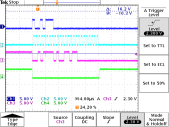
\includegraphics[width=0.6\textwidth]{ss_osc_adc_2v}
                \caption{Captura de osciloscopio de la conversión de 2V realizada por el ADC.}
                \label{fig:ss_osc_adc_2v}
            \end{figure} 

La conversión en el ADC comienza a partir del décimo pulso del dclk. En este caso, la conversión resultante fue 1001 1011 0000, lo que equivale a 2480 en decimal. Realizando una regla de tres, se obtiene que este valor corresponde a un voltaje de 1.9985V.


La segunda prueba consistió en aplicar 3.3V al canal 0 del ADC para evaluar su respuesta ante un voltaje mayor. En la siguiente figura se muestra la conversión resultante
            \begin{figure}[hbtp]
                \centering
                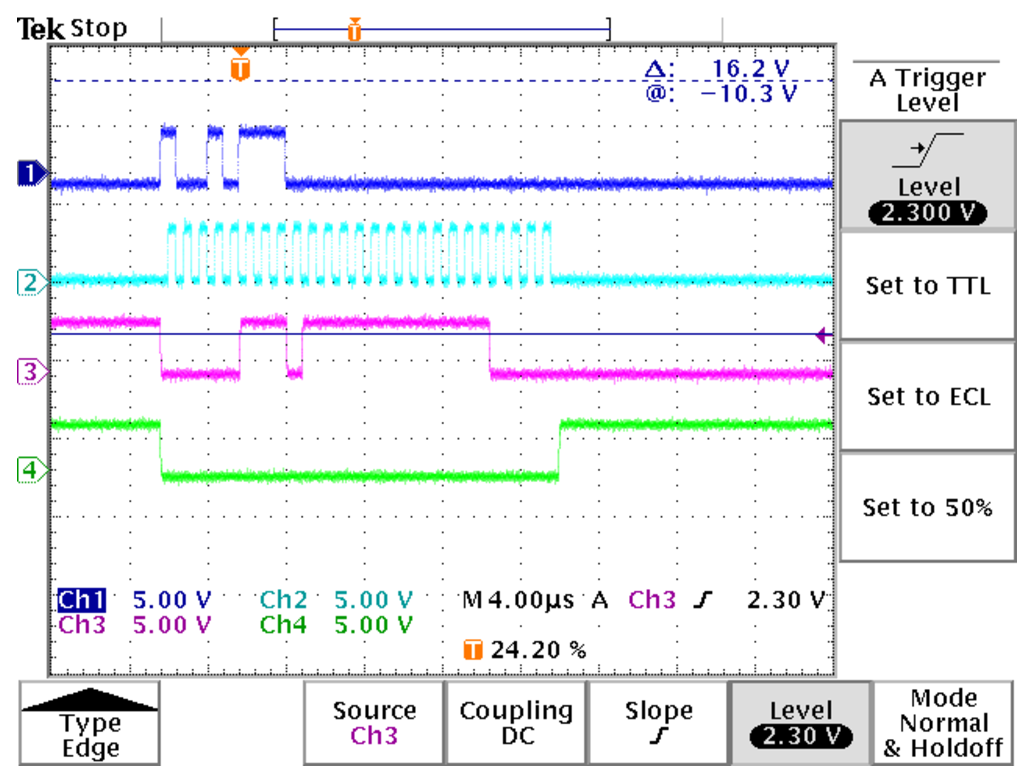
\includegraphics[width=0.6\textwidth]{ss_osc_adc_3v}
                \caption{Captura de osciloscopio de la conversión de 3.3V realizada por el ADC.}
                \label{fig:ss_osc_adc_3v}
            \end{figure} 

El resultado de la conversión fue 1111 1111 1111, que corresponde a 4095 en decimal. Este valor equivale a un voltaje de 3.3V, confirmando que el ADC realizó correctamente la conversión de la señal analógica al valor digital máximo posible para este canal.
     
\subsection{DAC}
Para controlar el DAC, se utilizó únicamente la escritura a través del protocolo SPI. Basándonos en el datasheet del DAC, la escritura se realiza en 16 ciclos de sck. Durante los primeros 4 ciclos, se envía el comando de configuración, en el cual se especifica en qué canal se tendrá el resultado de la conversión. En los 12 ciclos restantes, se transmite un valor de voltaje en formato binario de 12 bits al dispositivo para su conversión a señal analógica.


En las Figuras \ref{fig:ss_osc_dac_2v} y \ref{fig:ss_osc_dac_3v} se muestran las capturas del osciloscopio, donde se pueden observar tres señales numeradas del 1 al 3. La señal número 1 corresponde a los pulsos de reloj sck, la señal número 2 muestra el comando y el valor del voltaje en formato binario, y la señal número 3 representa el chip select del dispositivo. Todas estas señales fueron generadas por los módulos de diseño del protocolo SPI implementado.


Para verificar que el DAC realizara correctamente la conversión, se asignaron dos valores de voltaje en formato binario al MOSI: 1001 1011 0010, equivalente a 2V, y 1111 1111 1111, equivalente a 3.3V. Posteriormente, se midió el voltaje en el canal asignado utilizando un multímetro, confirmando que las conversiones fueron precisas.


En las siguientes imágenes se muestran las capturas del osciloscopio correspondientes a la escritura del DAC, así como el resultado de la conversión de 2V y 3.3V, respectivamente.

            \begin{figure}[hbtp]
                \centering
                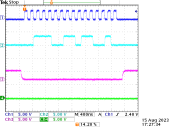
\includegraphics[width=0.6\textwidth]{ss_osc_dac_2v}
                \caption{Captura de osciloscopio de la escritura de 2V en binario en el DAC.}
                \label{fig:ss_osc_dac_2v}
            \end{figure}
            
            \begin{figure}[hbtp]
                \centering
                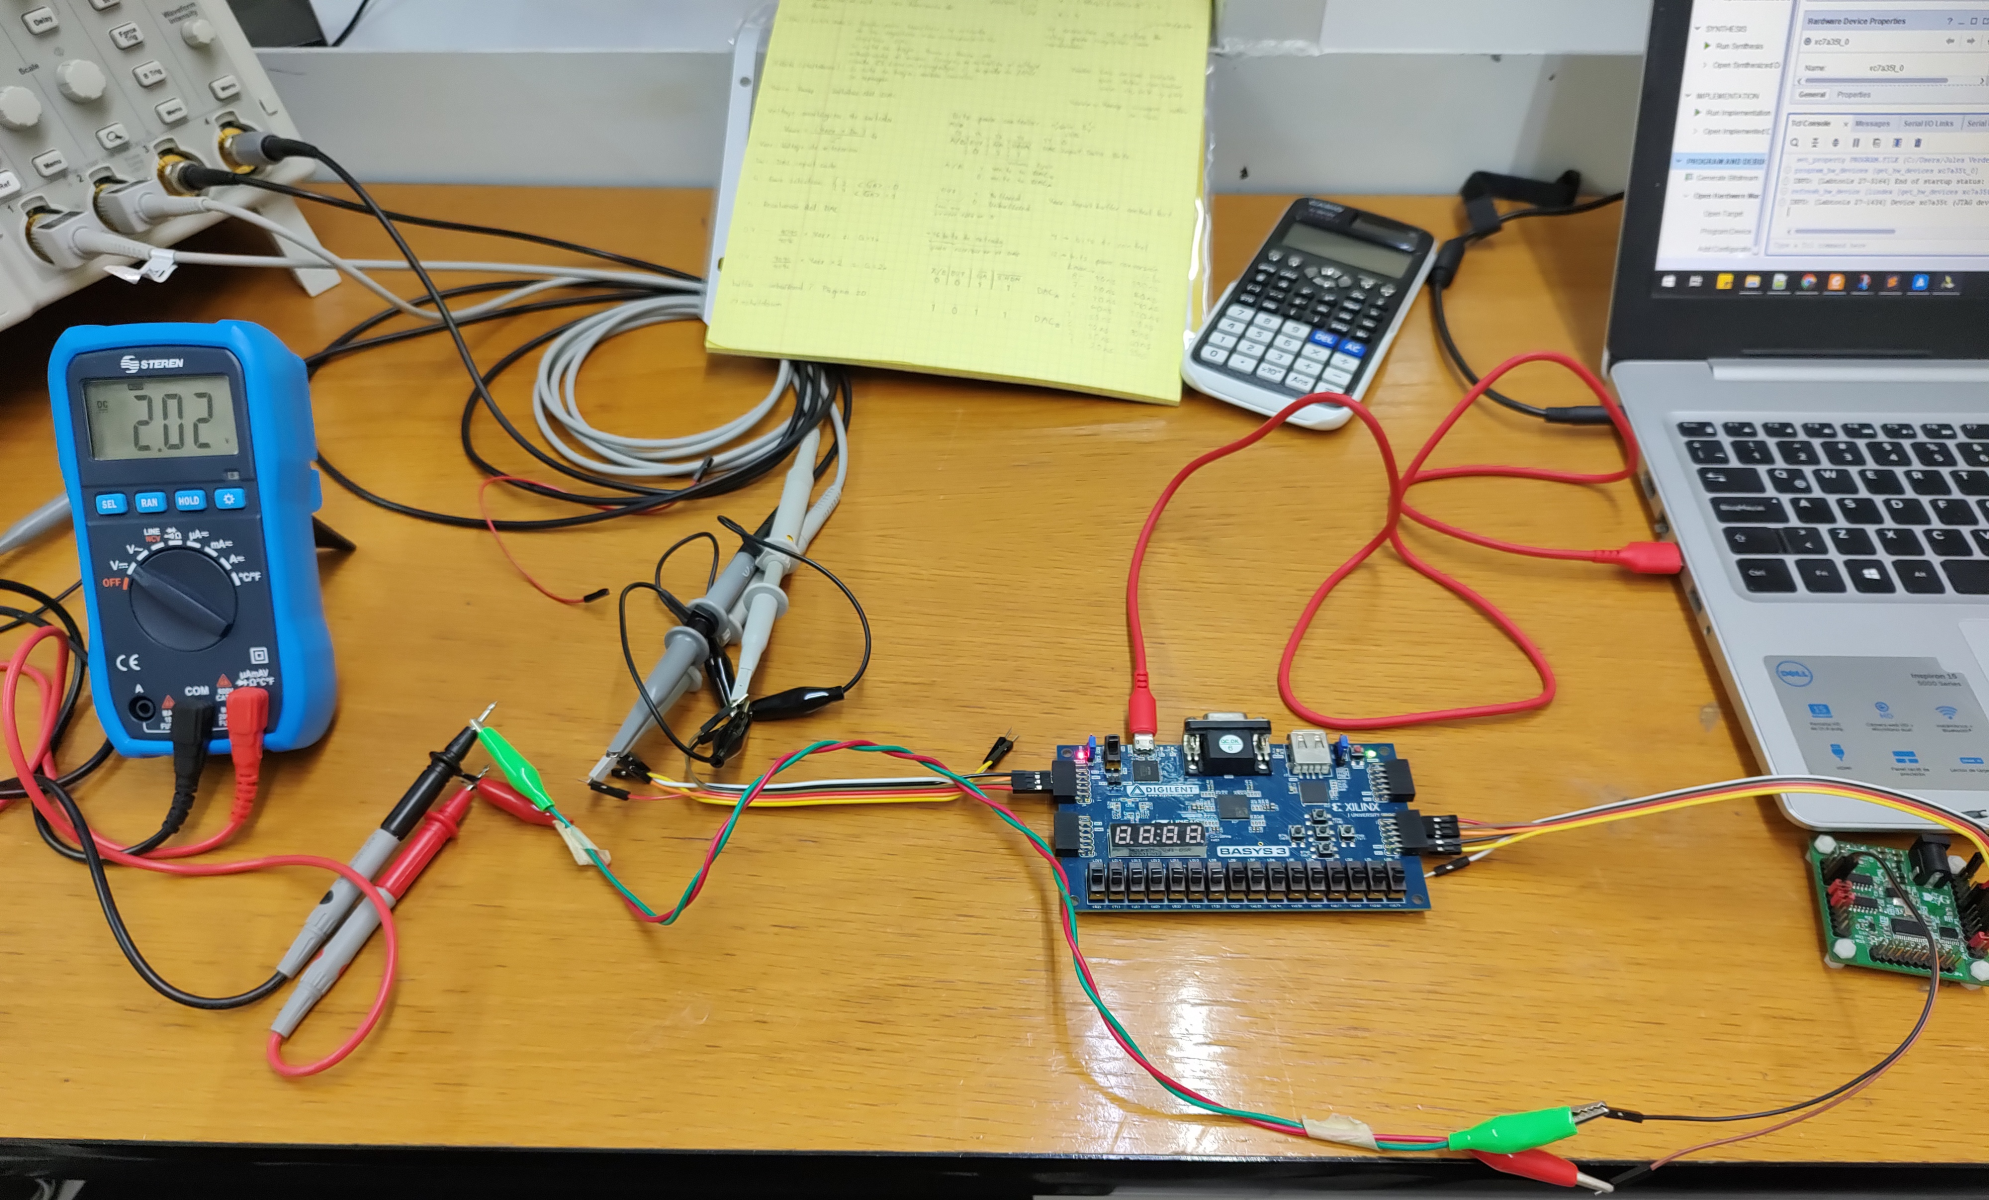
\includegraphics[width=0.6\textwidth]{dac_conversion_2v}
                \caption{Resultado de la conversión de 2V realizada por el DAC.}
                \label{fig:dac_conversion_2v}
            \end{figure}            
          
            \begin{figure}[hbtp]
                \centering
                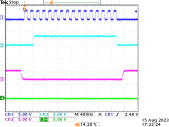
\includegraphics[width=0.6\textwidth]{ss_osc_dac_3v}
                \caption{Captura de osciloscopio de la escritura de 3.3V en binario en el DAC}
                \label{fig:ss_osc_dac_3v}
            \end{figure}   

            \begin{figure}[hbtp]
                \centering
                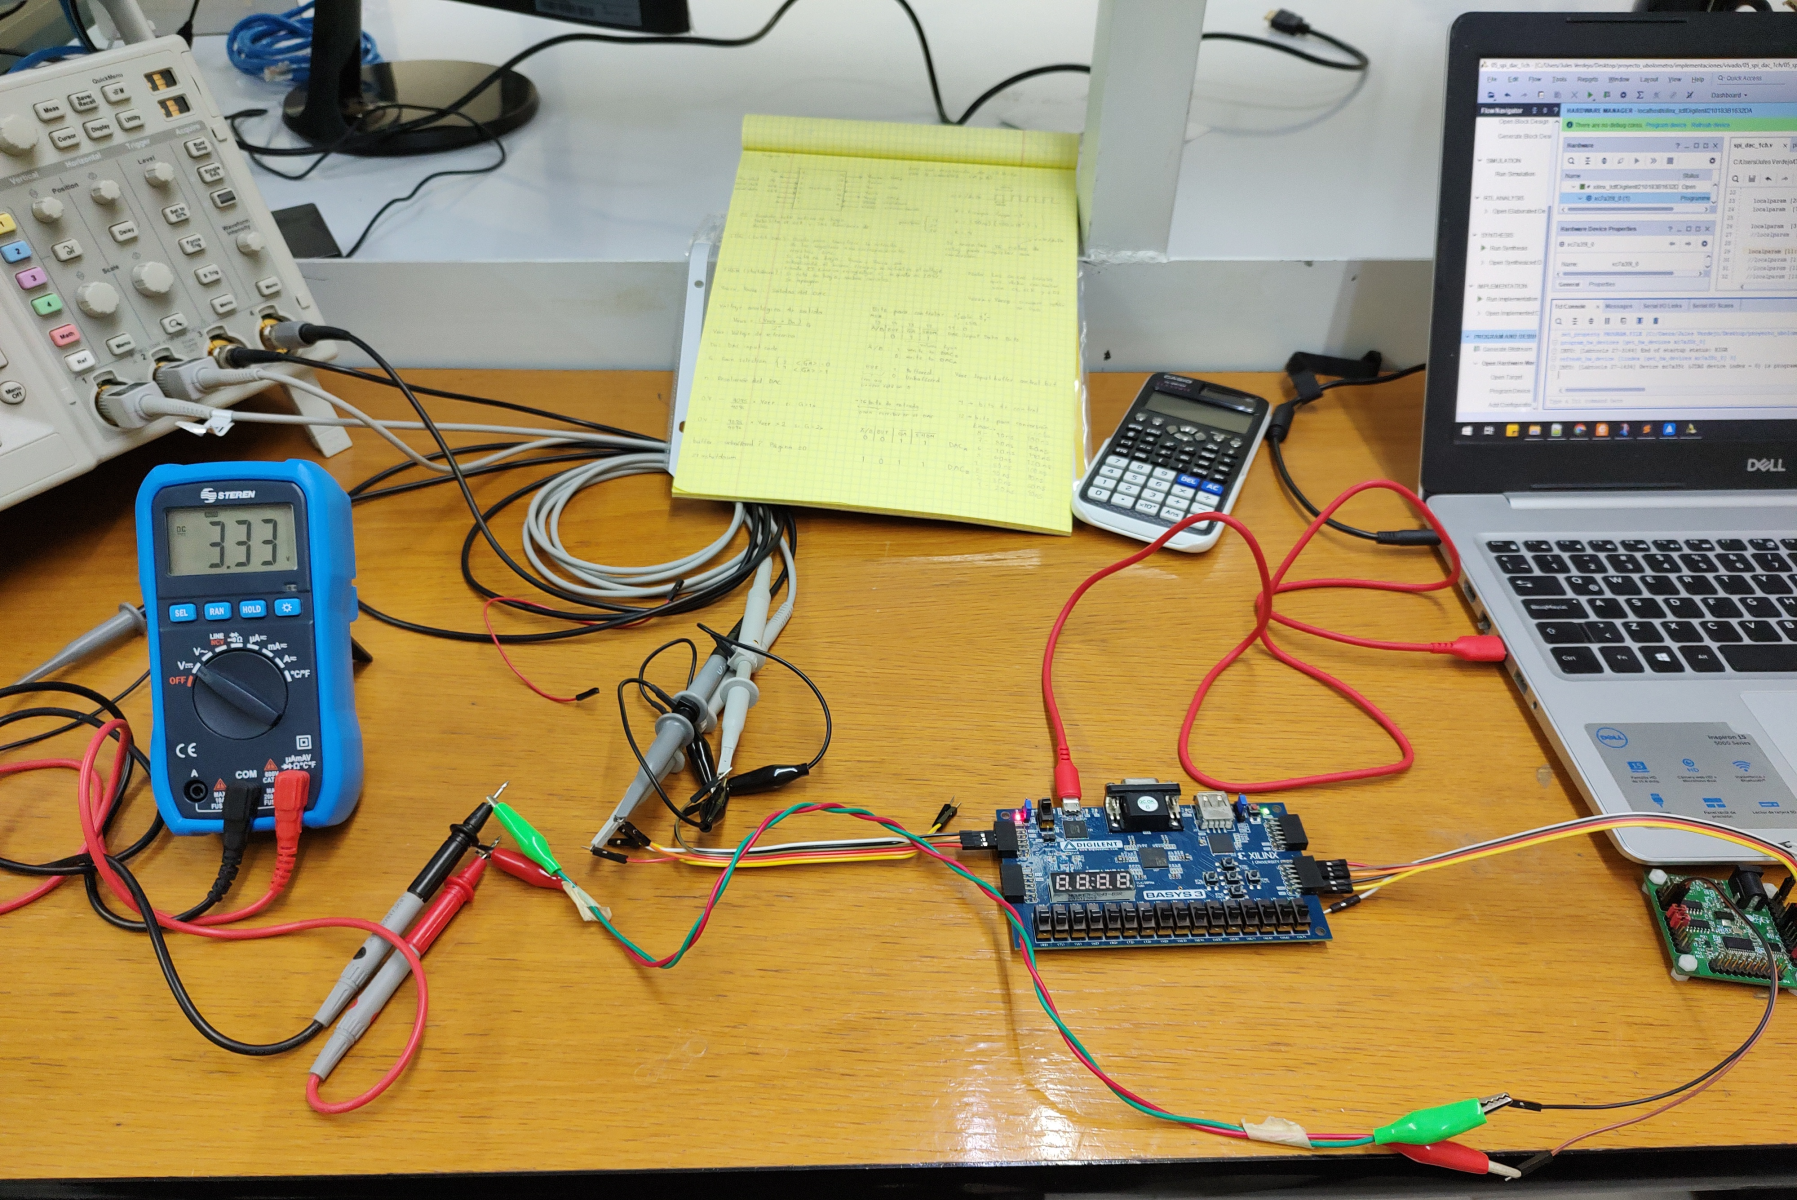
\includegraphics[width=0.6\textwidth]{dac_conversion_3v}
                \caption{Resultado de la conversión de 3.3V realizada por el DAC.}
                \label{fig:dac_conversion_3v}
            \end{figure} 
                                 
\section{Resultados de caracterización de resistencias}  
Al trabajar con la matriz de resistencias y al integrar los multiplexores en el sistema, se observó que el valor de voltaje recibido era menor de lo esperado. Este comportamiento anómalo llevó a sospechar que los multiplexores estaban introduciendo una resistencia adicional que afectaba las mediciones. Para investigar el impacto de esta resistencia en los resultados, se optó por medir la resistencia interna de los multiplexores. Esta medición permitió cuantificar el efecto de los multiplexores sobre los valores de voltaje obtenidos y ajustar el diseño para minimizar el impacto de esta resistencia en las lecturas.
            \begin{table}[htbp]
                \caption{Resistencia de multiplexores.}
                \begin{center}
                    \resizebox{0.9\linewidth}{!}{ 
                    \begin{NiceTabular}{| c | c | c | c | c | c |}
                        \CodeBefore
                        \Body
                        \hline
                        \textbf{$R_{test}$}  & \textbf{$V_{muxrows}$} & \textbf{$V_{muxcols}$} & \textbf{$i$} & \textbf{$R_{mux_{row}}$} & \textbf{$R_{mux_{col}}$}\\
                        \hline
                        1K$\Omega$   & 3.86e-2 V& 3.5e-2  V& 2.65e-4 A& 145.66 $\Omega$& 132$\Omega$\\
                        3.3K$\Omega$ & 3.43e-2 V& 3.1e-2  V& 2.21e-4 A& 155.2 $\Omega$& 140.27$\Omega$\\
                        5.6K$\Omega$ & 2.83e-2 V& 2.48e-2 V& 1.89e-4 A& 149.73 $\Omega$& 131.21$\Omega$\\
                        10K$\Omega$  & 2.25e-2 V& 2.11e-2 V& 1.49e-4 A& 151 $\Omega$& 141.6$\Omega$\\                            
                        \hline
                    \end{NiceTabular}
                    }
                \label{tab:Mux_res}
                \end{center}
            \end{table}

            \begin{figure}[hbtp]
                \centering
                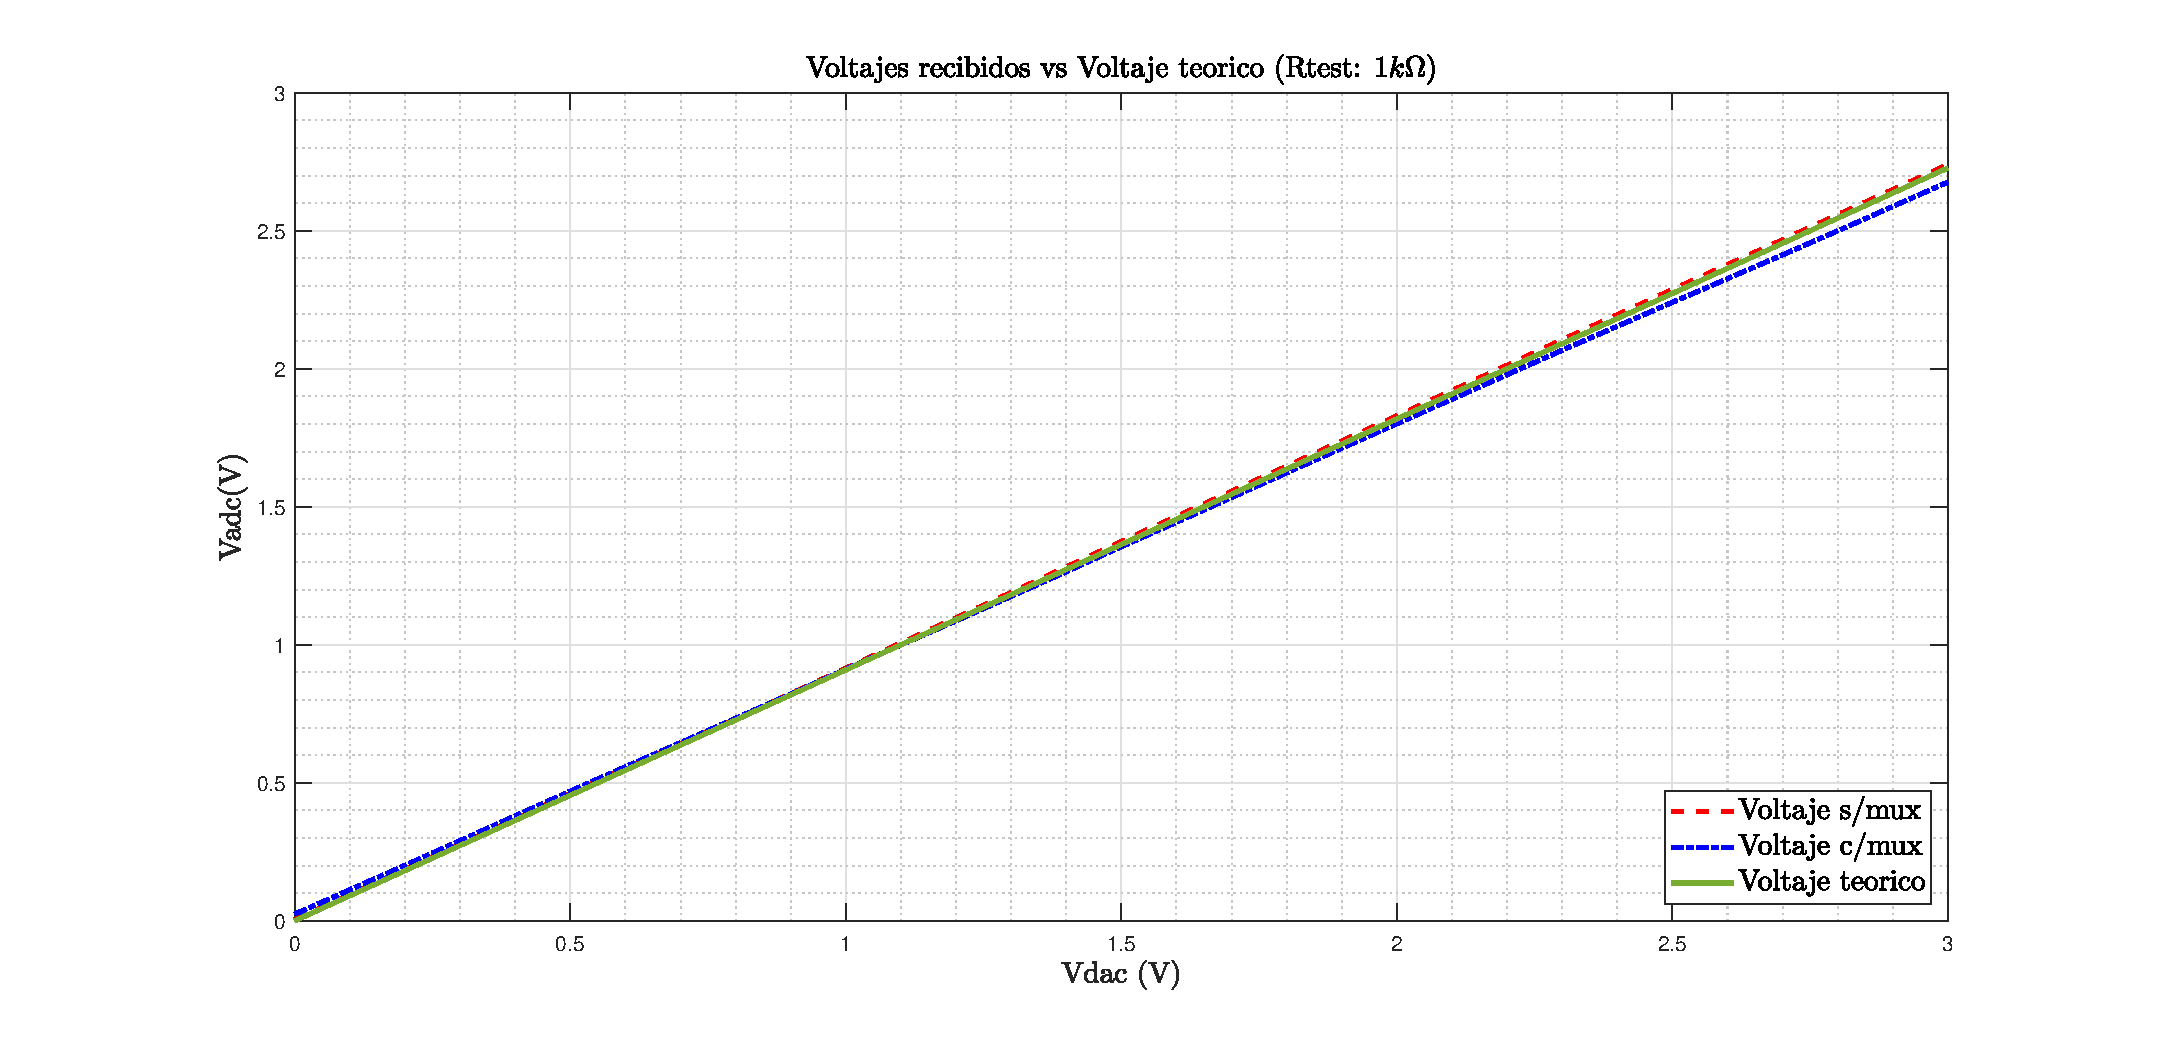
\includegraphics[width=1\textwidth]{01_1k}
                \caption{Influencia de resistencia de multiplexores.}
                \label{fig:01_1k}
            \end{figure}  
            
            \begin{figure}[hbtp]
                \centering
                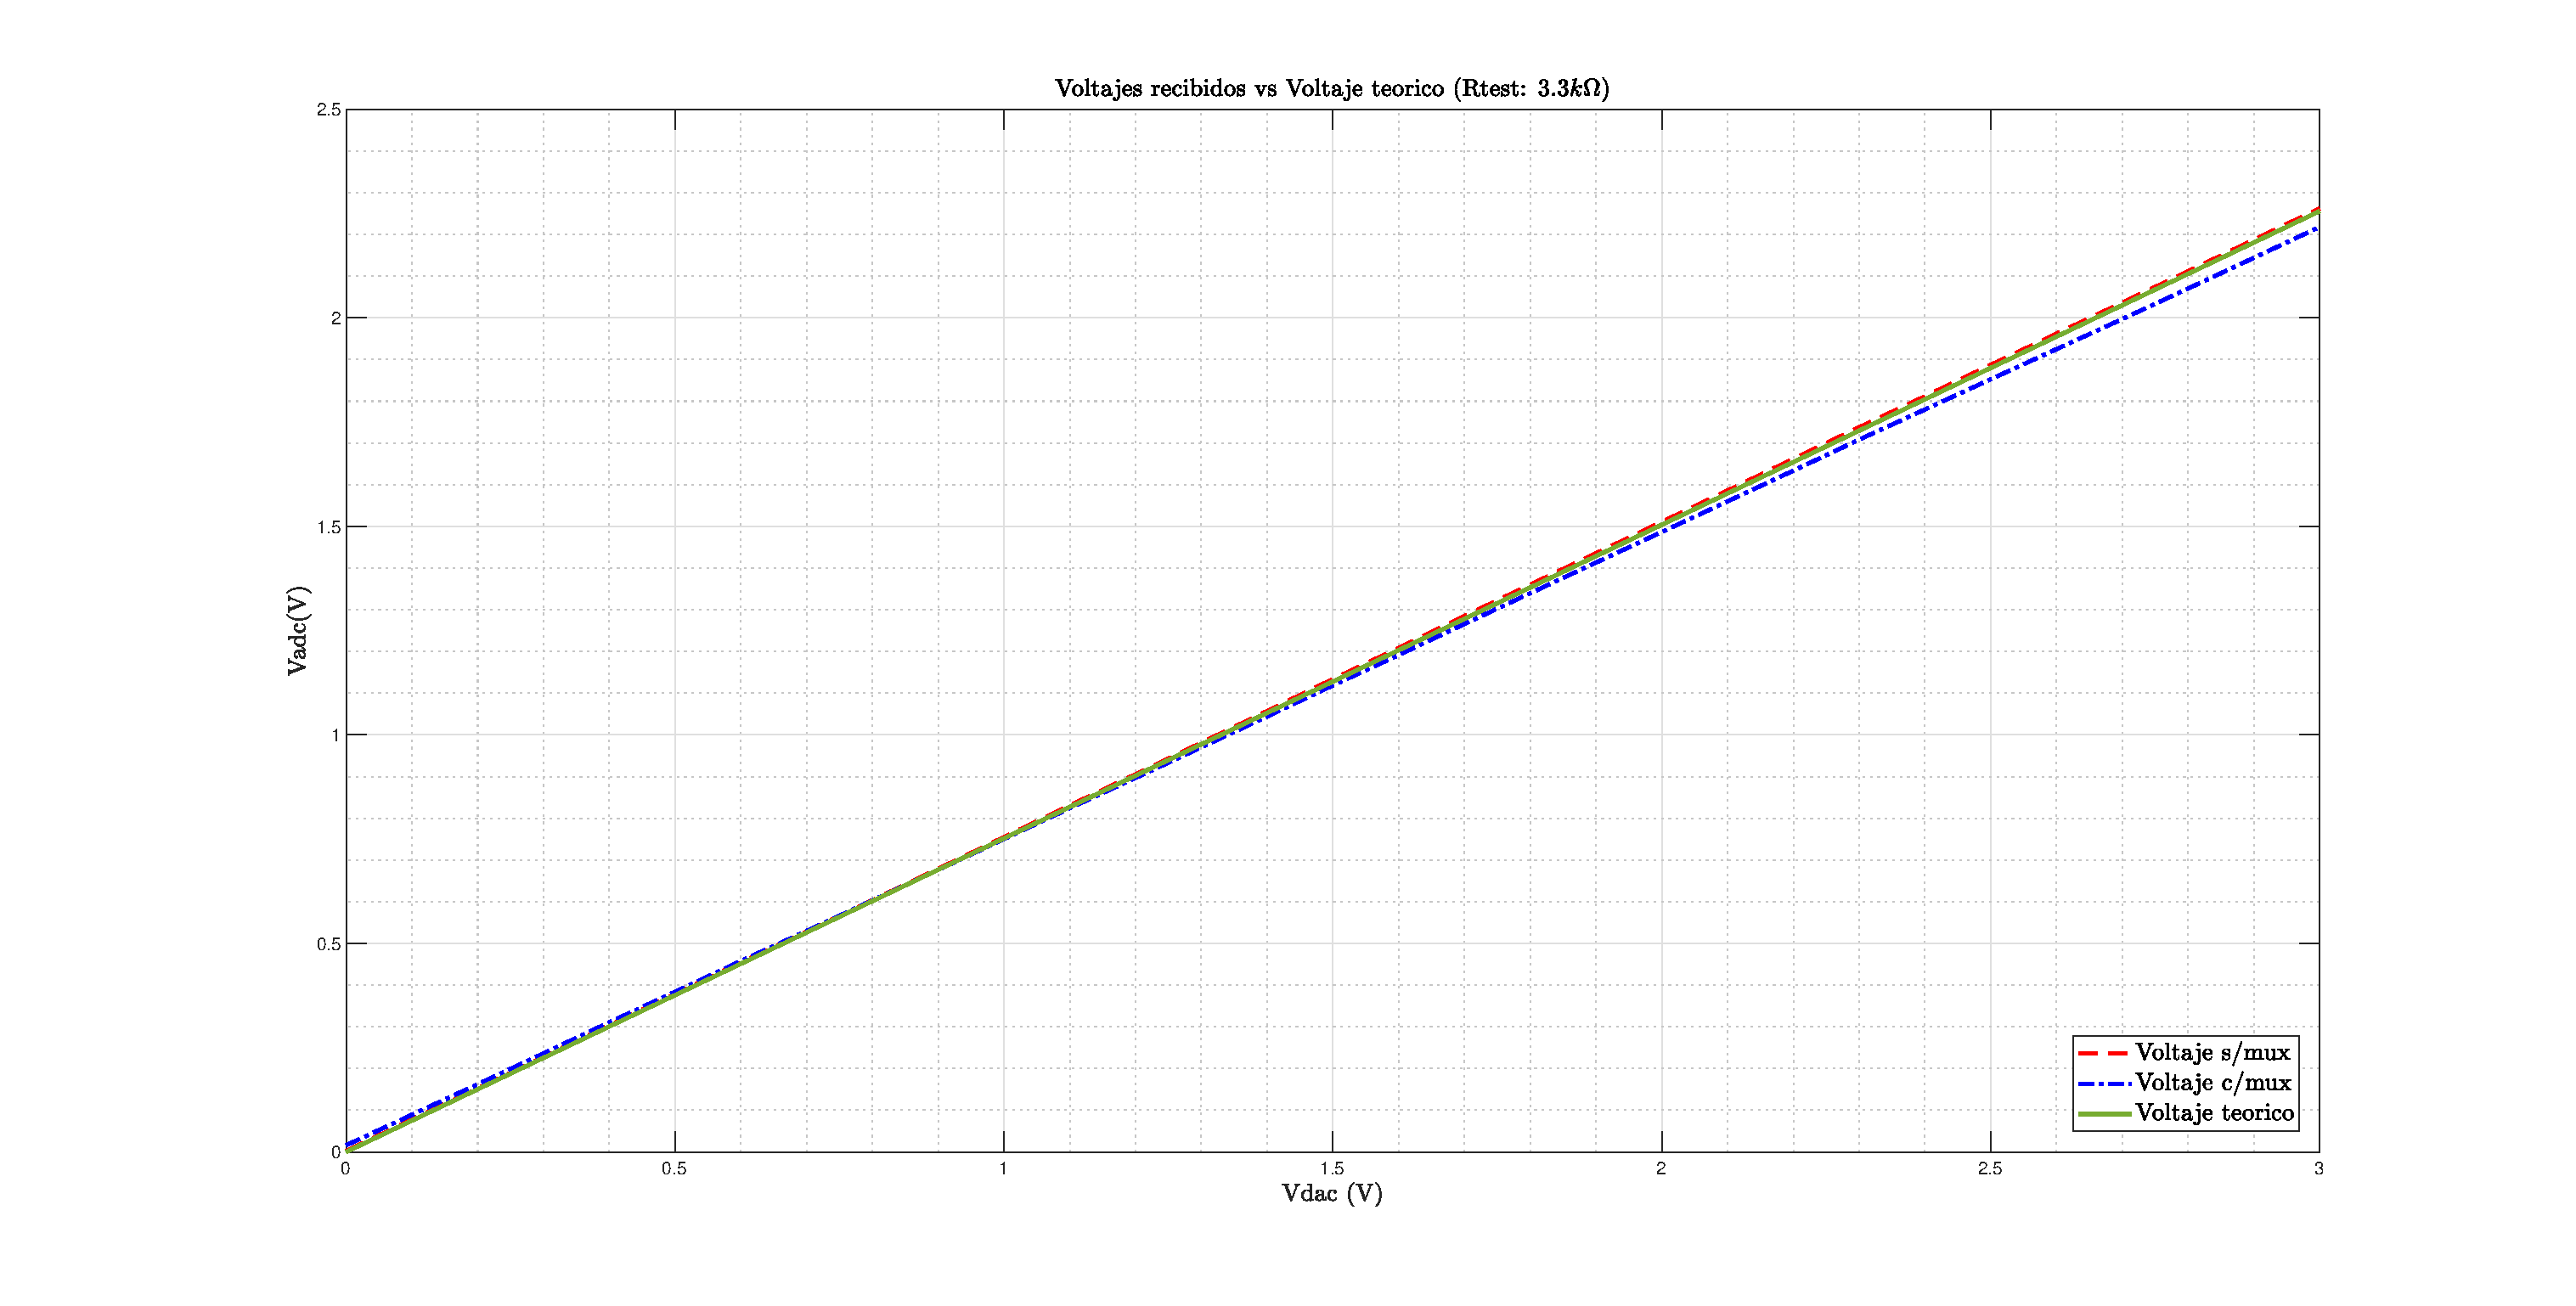
\includegraphics[width=1\textwidth]{02_3k3_new}
                \caption{Influencia de resistencia de multiplexores.}
                \label{fig:02_3k3_new}
            \end{figure}              
 
            \begin{figure}[hbtp]
                \centering
                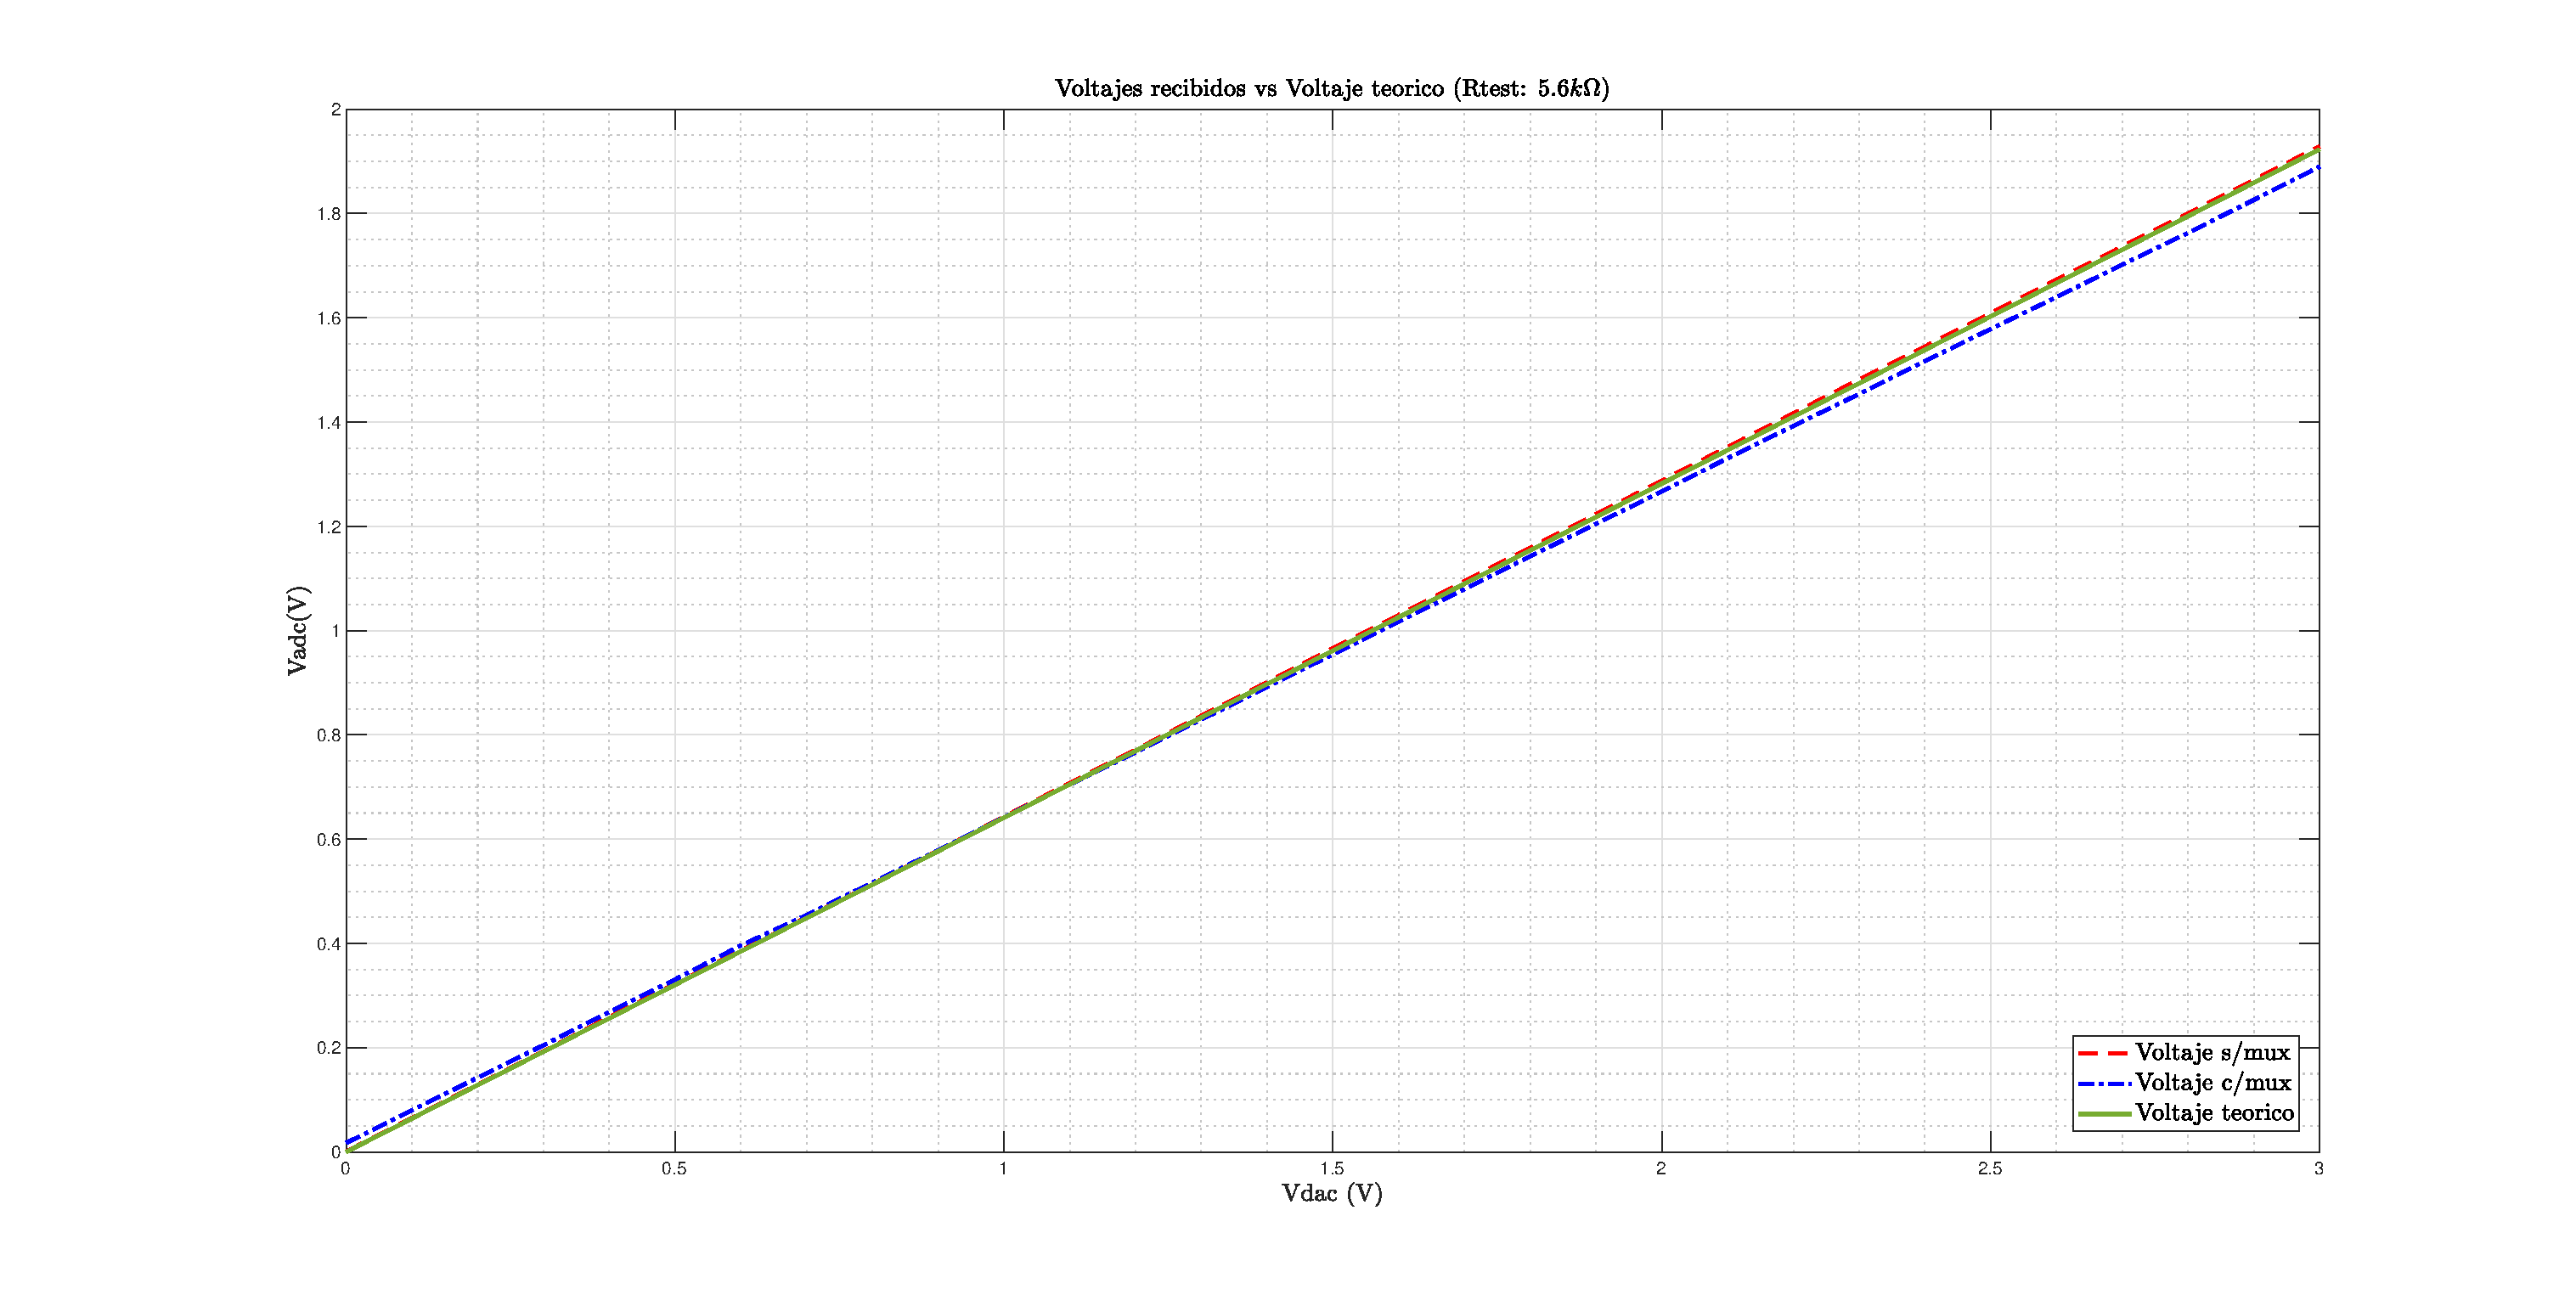
\includegraphics[width=1\textwidth]{03_5k6_new}
                \caption{Influencia de resistencia de multiplexores.}
                \label{fig:03_5k6_new}
            \end{figure}   

            \begin{figure}[hbtp]
                \centering
                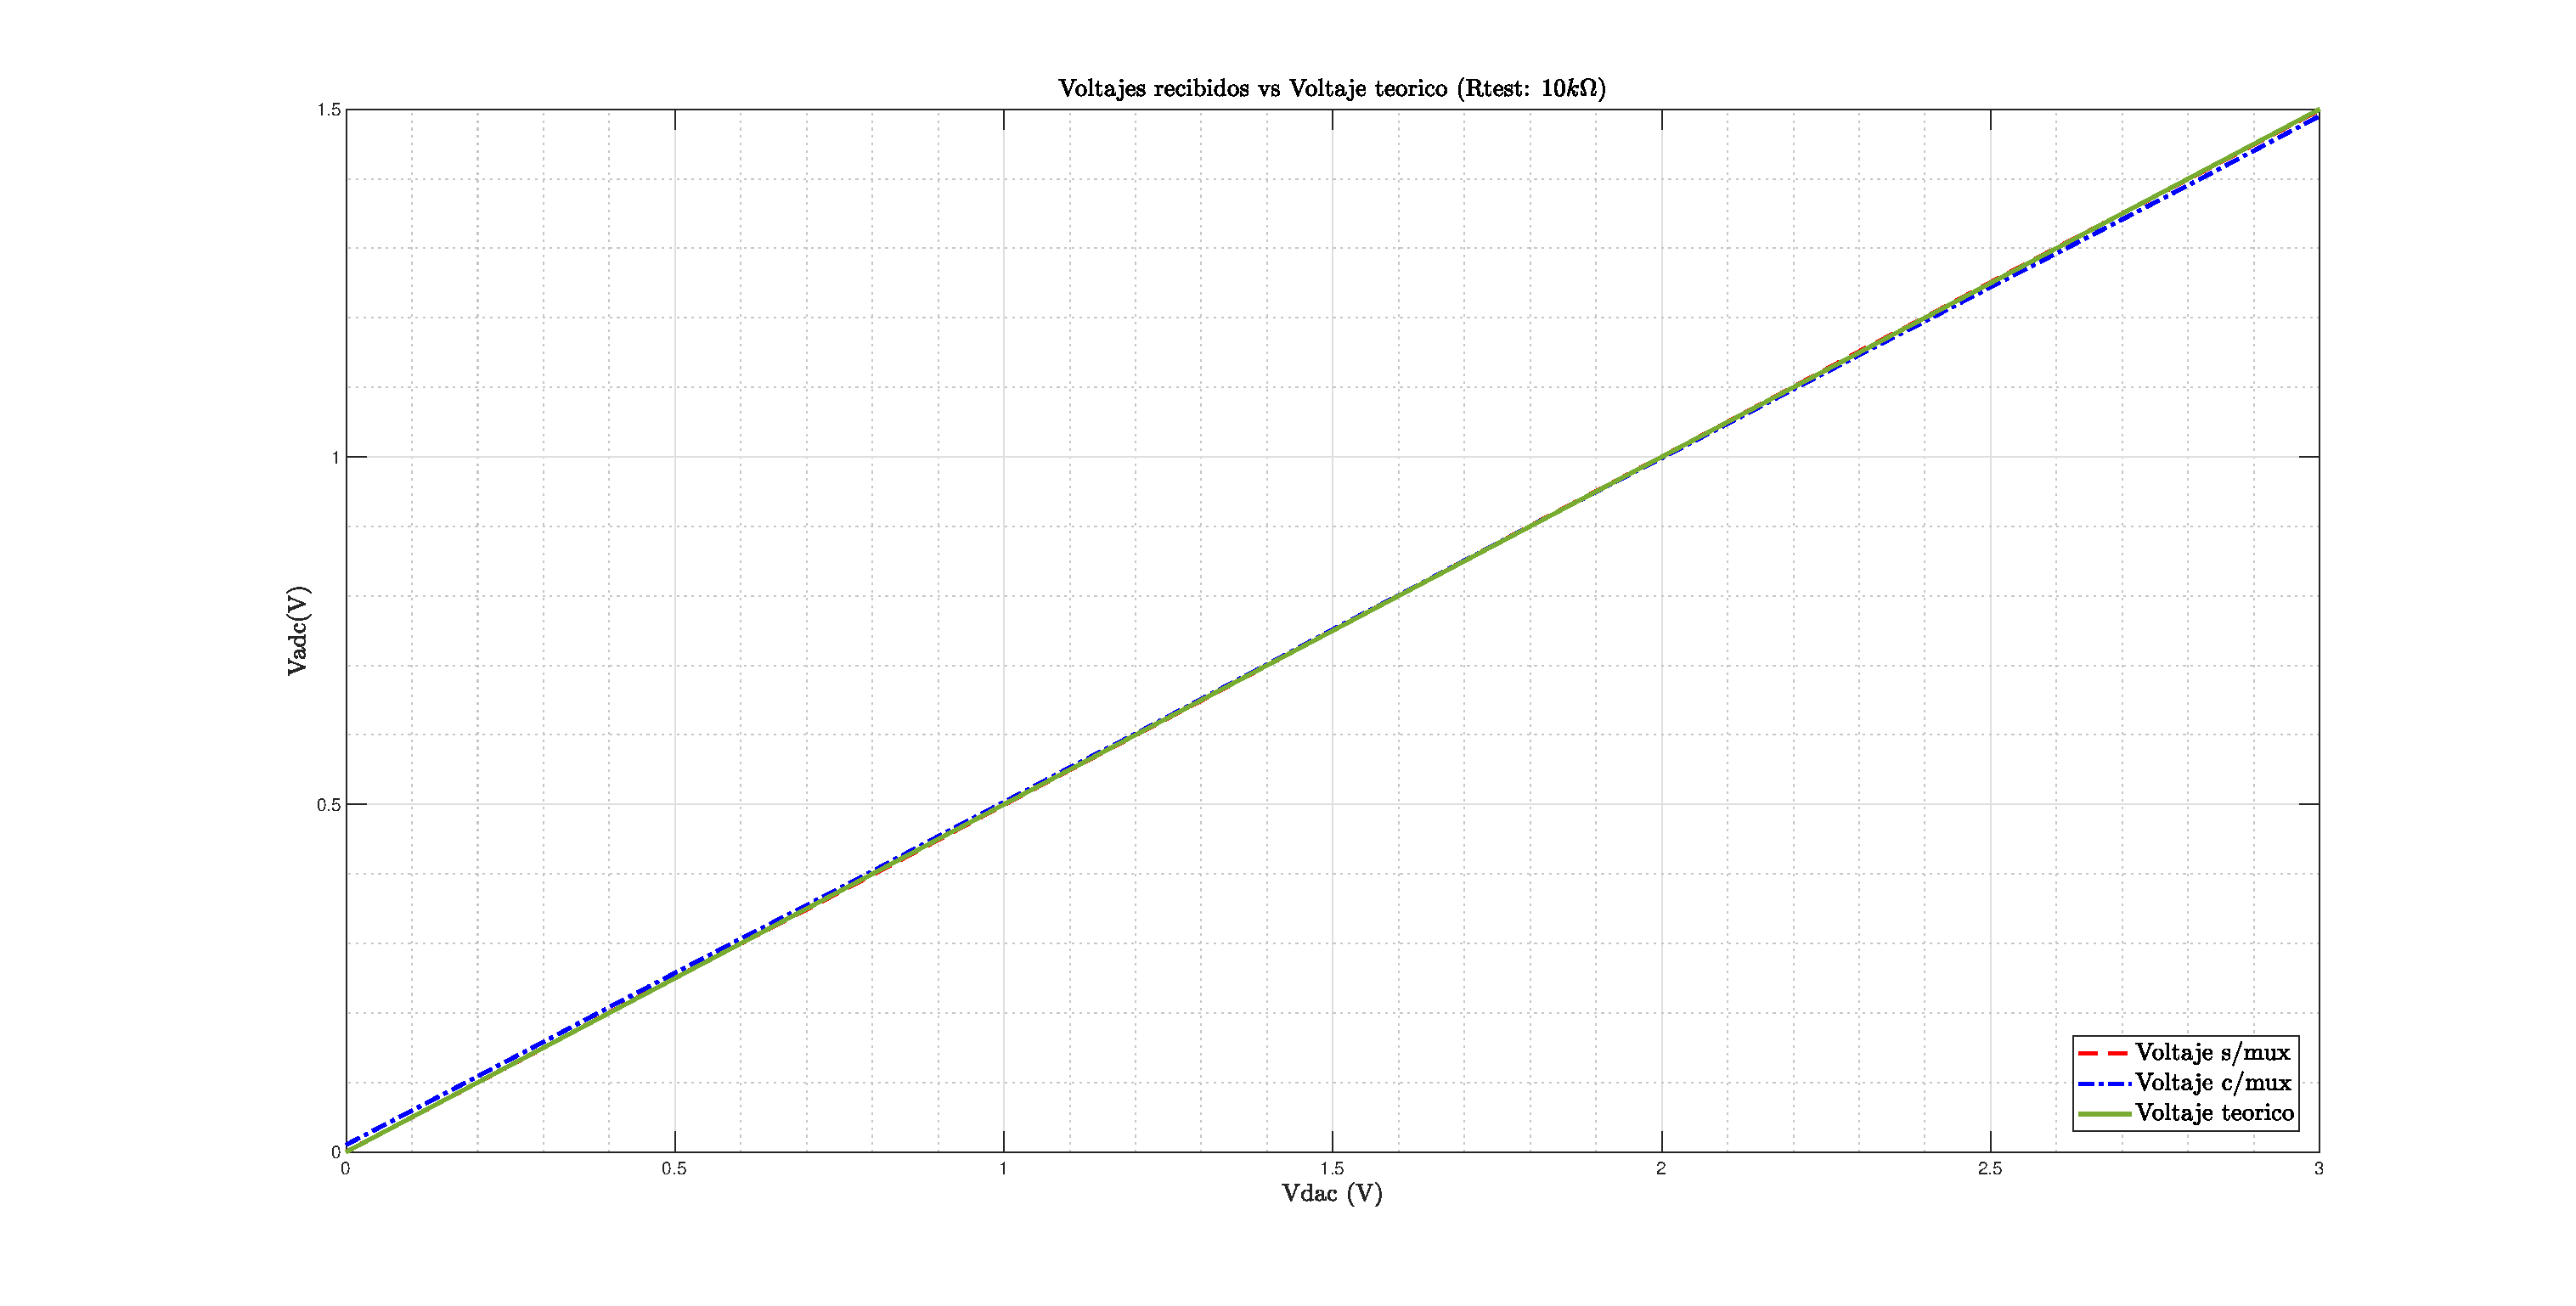
\includegraphics[width=1\textwidth]{04_10k_new}
                \caption{Influencia de resistencia de multiplexores.}
                \label{fig:04_10k_new}
            \end{figure}  
                
                     
\section{Resultados de caracterización de fotorresistencias}

            \begin{table}[htbp]
                \caption{Valor de fotorresistencias con diferentes duty cycles.}
                \begin{center}
                    \resizebox{0.6\linewidth}{!}{ 
                    \begin{NiceTabular}{| c | c | c |}
                        \CodeBefore
                        \Body
                        \hline
                        \textbf{$V_{Fuente}$}  & \textbf{Duty cycle ($\%$)} & \textbf{$R_{med} (K\Omega)$} \\
                        \hline
                        3 V     & 25  & 210 - 213.7\\
                                & 50  & 104 - 105.7\\
                                & 75  & 70 -71\\
                                & 100 & 53 - 54\\ \hline
                        3.3 V   & 25  & 29 - 31\\
                                & 50  & 16 - 17\\
                                & 75  & 11 - 12\\
                                & 100 & 8 - 9\\ \hline
                        3.5 V   & 25  & 6 - 7\\
                                & 50  & 3.6\\
                                & 75  & 2.6\\
                                & 100 & 2\\                             
                        \hline
                    \end{NiceTabular}
                    }
                \label{tab:Duty_cycle}
                \end{center}
            \end{table}


            \begin{figure}[hbtp]
                \centering
                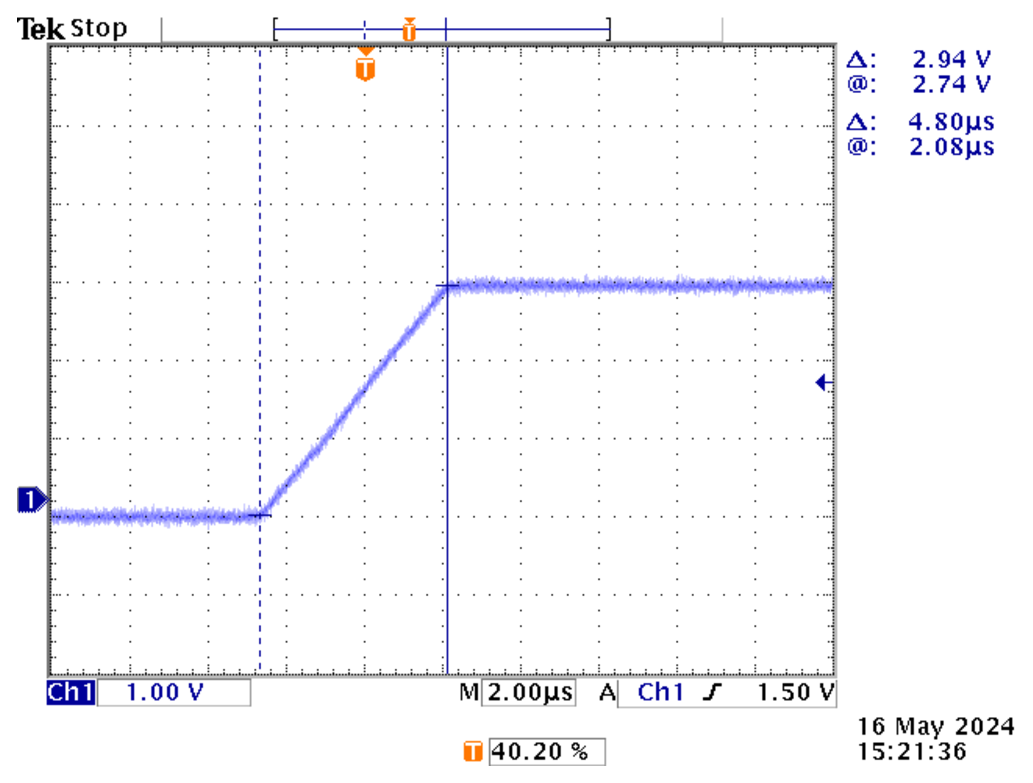
\includegraphics[width=0.6\textwidth]{settling_3v}
                \caption{Captura de osciloscopio de settling time.}
                \label{fig:settling_3v}
            \end{figure}
            
            \begin{figure}[hbtp]
                \centering
                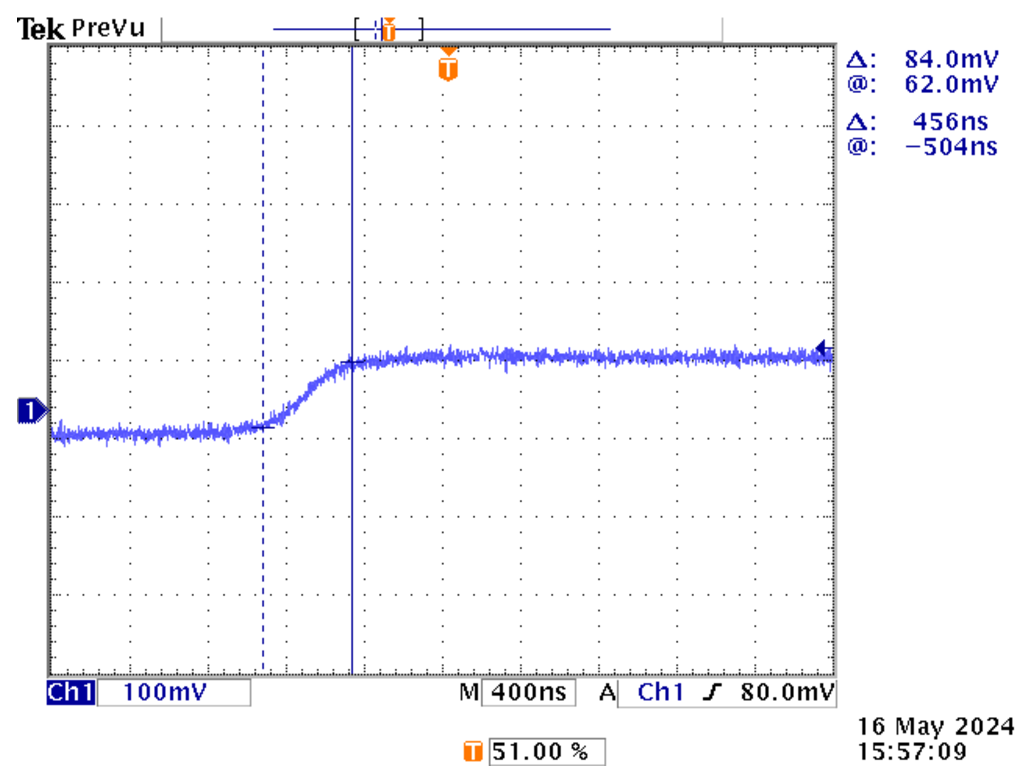
\includegraphics[width=0.6\textwidth]{settling_0v1}
                \caption{Captura de osciloscopio de settling time.}
                \label{fig:settling_0v1}
            \end{figure} 
            
            \begin{figure}[hbtp]
                \centering
                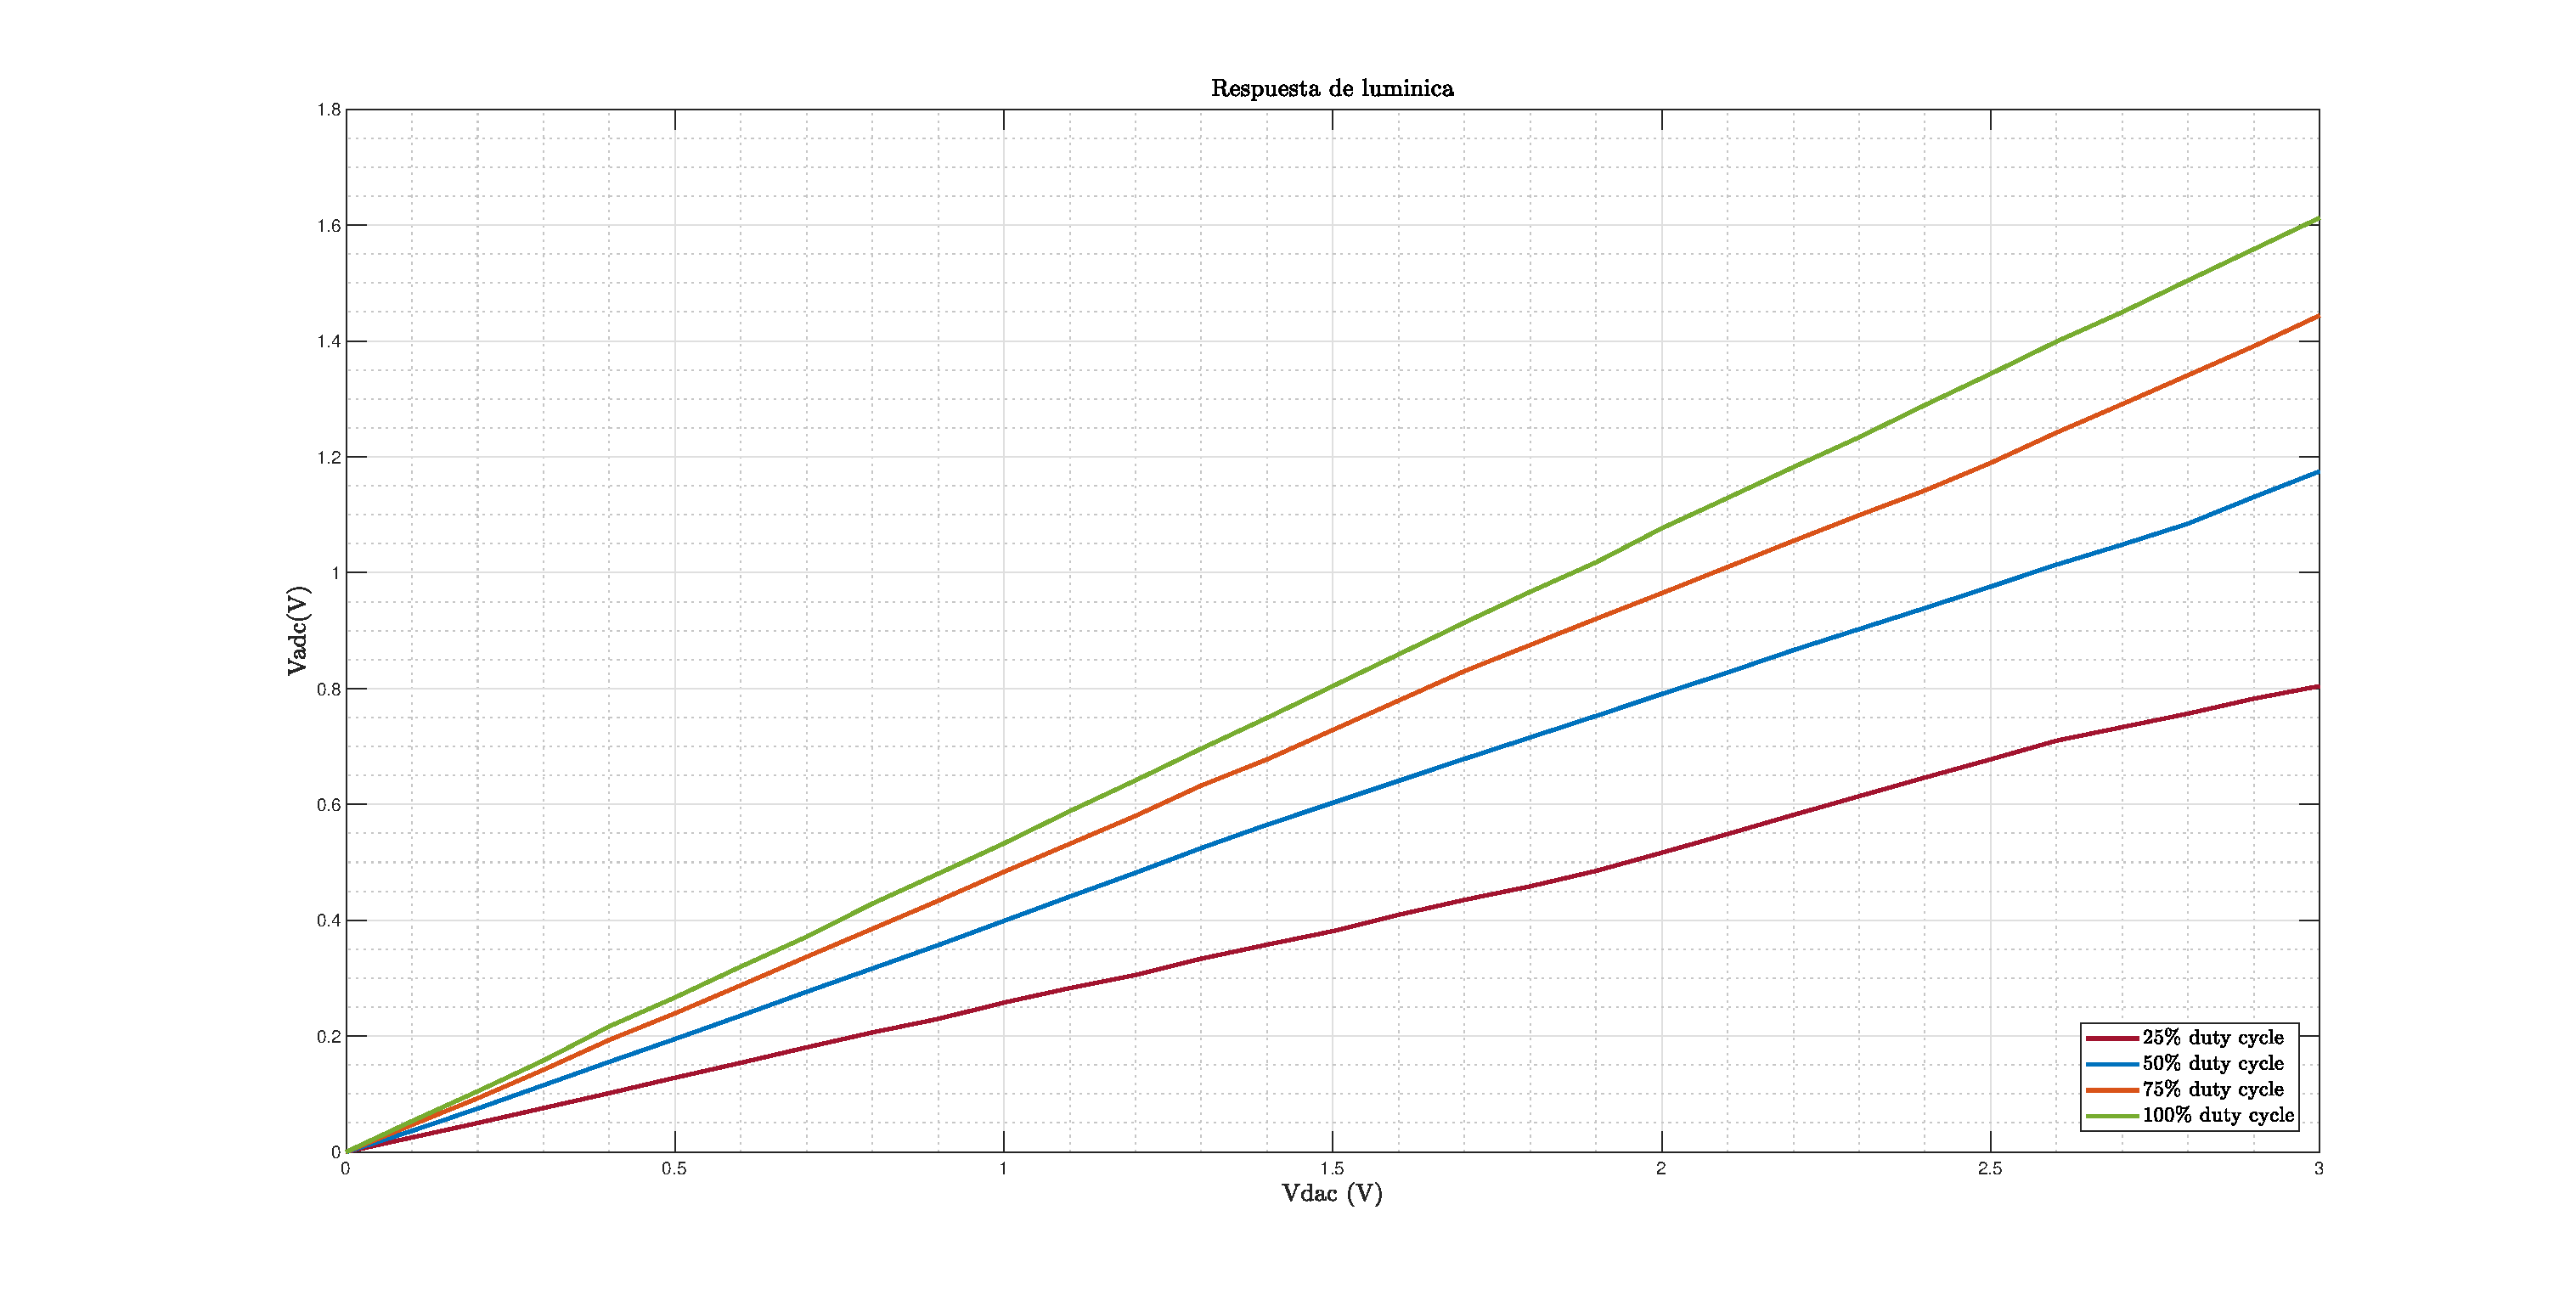
\includegraphics[width=1\textwidth]{respuesta_luminica}
                \caption{Respuesta lumínica.}
                \label{fig:respuesta_luminica}
            \end{figure}            
            
            

\section{Imágenes obtenidas}

            \begin{figure}[hbtp]
                \centering
                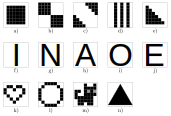
\includegraphics[width=0.8\textwidth]{mask_final}
                \caption{Máscaras aplicadas a matriz de fototransistores.}
                \label{fig:mask_final}
            \end{figure}  

            \begin{figure}[hbtp]
                \centering
                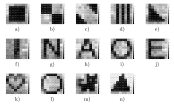
\includegraphics[width=0.8\textwidth]{result_mask}
                \caption{Resultados de las máscaras aplicadas a los fototransistores.}
                \label{fig:result_mask}
            \end{figure}

	\chapter{Conclusiones}

\begin{itemize}
 \item Uno de los principales logros de este trabajo fue el diseño de códigos robustos, modulares y escalables para la implementación del protocolo SPI en Verilog, específicamente para el control de los convertidores analógico-digital (A/D) y digital-analógico (D/A), ADS7841 y MCP4922, respectivamente. La robustez del SPI fue comprobada a través de simulaciones, mediciones con osciloscopio y multímetro, así como por la recepción de datos mediante MATLAB. Estos códigos no solo cumplen con los requisitos del proyecto, sino que además tienen la flexibilidad de ser reutilizados y adaptados a futuras necesidades. Su diseño modular permite modificaciones fáciles y rápidas.
 \item Se logró diseñar una PCB funcional con una matriz de 8x8 fototransistores, capaz de detectar las variaciones de luz. La PCB no solo demostró ser eficiente en su propósito, sino que también cumplió con todos los requisitos de diseño y fabricación, lo que permitió que fuera producida y ensamblada exitosamente. Este resultado valida tanto el diseño como su implementación práctica, asegurando su utilidad en aplicaciones futuras que requieran la captura de imágenes a través de variaciones lumínicas.  
 \item El módulo de caracterización desarrollado no solo demostró ser eficaz para las pruebas realizadas, sino que también ofrece la flexibilidad necesaria para ser modificado y adaptado para la caracterización de un microbolómetro real. Este enfoque modular permite que el sistema se ajuste a diferentes requisitos y aplicaciones.
 \item Aunque en este trabajo el uso de una resistencia de referencia y un capacitor fueron suficientes para emplearse como circuito de lectura, no significa que estos vayan a servir para un cualquier tipo de sensor. Es necesario contar con un circuito de lectura específico adaptado a la señal de salida generada por el detector en uso. Esto es esencial para asegurar una captura precisa y eficiente de los datos.
 \item Para obtener lecturas adecuadas de una matriz de detectores, no es suficiente contar únicamente con convertidores A/D y D/A de alta resolución. Es igualmente crucial utilizar multiplexores que no introduzcan una resistencia excesiva en el circuito. La resistencia añadida por los multiplexores altera las mediciones, afectando la precisión del sistema de adquisición de datos. Por lo tanto, es esencial seleccionar cuidadosamente los componentes para minimizar estas interferencias y obtener lecturas precisas y confiables.
\end{itemize}


    


\appendix
	\chapter{Códigos}

%\lstinputlisting[style = MATLAB, caption =  Nombre de abajo, label = cod:nombre1]{codigos/matlab/test_code.m}

	\section{Códigos en C}
%\lstinputlisting[style = C, caption =  Comprobar el número de bytes de los tipos de dato del sistema., label = cod:A1]{codigos/c_codes/A1_check_sys_bytes.c}



\backmatter

%\nocite{*}
\bibliographystyle{ieeetr}
\bibliography{bibliografia2}

\end{document}
